\documentclass[11pt]{article}\usepackage[]{graphicx}\usepackage[]{color}
%% maxwidth is the original width if it is less than linewidth
%% otherwise use linewidth (to make sure the graphics do not exceed the margin)
\makeatletter
\def\maxwidth{ %
  \ifdim\Gin@nat@width>\linewidth
    \linewidth
  \else
    \Gin@nat@width
  \fi
}
\makeatother

\definecolor{fgcolor}{rgb}{0.345, 0.345, 0.345}
\newcommand{\hlnum}[1]{\textcolor[rgb]{0.686,0.059,0.569}{#1}}%
\newcommand{\hlstr}[1]{\textcolor[rgb]{0.192,0.494,0.8}{#1}}%
\newcommand{\hlcom}[1]{\textcolor[rgb]{0.678,0.584,0.686}{\textit{#1}}}%
\newcommand{\hlopt}[1]{\textcolor[rgb]{0,0,0}{#1}}%
\newcommand{\hlstd}[1]{\textcolor[rgb]{0.345,0.345,0.345}{#1}}%
\newcommand{\hlkwa}[1]{\textcolor[rgb]{0.161,0.373,0.58}{\textbf{#1}}}%
\newcommand{\hlkwb}[1]{\textcolor[rgb]{0.69,0.353,0.396}{#1}}%
\newcommand{\hlkwc}[1]{\textcolor[rgb]{0.333,0.667,0.333}{#1}}%
\newcommand{\hlkwd}[1]{\textcolor[rgb]{0.737,0.353,0.396}{\textbf{#1}}}%

\usepackage{framed}
\makeatletter
\newenvironment{kframe}{%
 \def\at@end@of@kframe{}%
 \ifinner\ifhmode%
  \def\at@end@of@kframe{\end{minipage}}%
  \begin{minipage}{\columnwidth}%
 \fi\fi%
 \def\FrameCommand##1{\hskip\@totalleftmargin \hskip-\fboxsep
 \colorbox{shadecolor}{##1}\hskip-\fboxsep
     % There is no \\@totalrightmargin, so:
     \hskip-\linewidth \hskip-\@totalleftmargin \hskip\columnwidth}%
 \MakeFramed {\advance\hsize-\width
   \@totalleftmargin\z@ \linewidth\hsize
   \@setminipage}}%
 {\par\unskip\endMakeFramed%
 \at@end@of@kframe}
\makeatother

\definecolor{shadecolor}{rgb}{.97, .97, .97}
\definecolor{messagecolor}{rgb}{0, 0, 0}
\definecolor{warningcolor}{rgb}{1, 0, 1}
\definecolor{errorcolor}{rgb}{1, 0, 0}
\newenvironment{knitrout}{}{} % an empty environment to be redefined in TeX

\usepackage{alltt}
\usepackage{amsmath}
\usepackage{listings}
\usepackage{stmaryrd}
\usepackage{bbm}
\usepackage{amsmath}
\usepackage{mathtools}
\usepackage{pdfpages}
\usepackage{breqn}
\usepackage[utf8]{inputenc}


\newcount\colveccount
\newcommand*\colvec[1]{
        \global\colveccount#1
        \begin{pmatrix}
        \colvecnext
}
\def\colvecnext#1{
        #1
        \global\advance\colveccount-1
        \ifnum\colveccount>0
                \\
                \expandafter\colvecnext
        \else
                \end{pmatrix}
        \fi
}
\newcommand{\argmin}{\arg\!\min}

\author{Thibault Doutre, Student ID 26980469}
\title{STAT230 HW 11 \\
University of California, Berkeley}
\date{\today}
\IfFileExists{upquote.sty}{\usepackage{upquote}}{}
\begin{document}

\maketitle
I would like to thank Shamindra for discussing the project with me.
\section{}
\subsection{Load data}
\begin{knitrout}
\definecolor{shadecolor}{rgb}{0.969, 0.969, 0.969}\color{fgcolor}\begin{kframe}
\begin{alltt}
\hlkwd{rm}\hlstd{(}\hlkwc{list} \hlstd{=} \hlkwd{ls}\hlstd{())}
\hlkwd{cat}\hlstd{(}\hlstr{"\textbackslash{}014"}\hlstd{)}
\end{alltt}
\end{kframe}\begin{kframe}\begin{alltt}
\hlcom{# Data -----------------------------------------------------}

\hlstd{makedata}\hlkwb{=}\hlkwa{function}\hlstd{(}\hlkwc{p}\hlstd{=}\hlnum{20}\hlstd{,}\hlkwc{wh}\hlstd{=}\hlnum{15}\hlstd{,}\hlkwc{n}\hlstd{=}\hlnum{100}\hlstd{)\{}
\hlcom{# This function generates p independent X variables and then uses wh of them}
\hlcom{# to generate Y based on coefficients determined by exp(exps) below.}
\hlcom{# Outside of the function, the data frame named data is further changed to}
\hlcom{# randomize the order of the variables so it's hard to tell for sure which}
\hlcom{# ones were used to generate Y.  You can always go back and examine switch}
\hlcom{# to figure out if your models include the right variables and which ones.}
  \hlstd{X}\hlkwb{=}\hlkwd{matrix}\hlstd{(}\hlkwd{rnorm}\hlstd{(n}\hlopt{*}\hlstd{p),n,p)}
  \hlstd{exps}\hlkwb{=}\hlkwd{seq}\hlstd{(}\hlopt{-}\hlnum{1}\hlstd{,}\hlopt{-}\hlnum{2.5}\hlstd{,}\hlkwc{length}\hlstd{=wh)}
  \hlstd{beta}\hlkwb{=}\hlkwd{rep}\hlstd{(}\hlnum{0}\hlstd{,p)}
  \hlstd{beta[}\hlnum{1}\hlopt{:}\hlstd{wh]}\hlkwb{=}\hlkwd{exp}\hlstd{(exps)}
  \hlstd{Y}\hlkwb{=}\hlnum{.5}\hlopt{+}\hlstd{X}\hlopt\hlstd{beta}\hlopt{+}\hlkwd{rnorm}\hlstd{(n)}
  \hlstd{data} \hlkwb{=} \hlkwd{data.frame}\hlstd{(Y,X)}
  \hlkwd{colnames}\hlstd{(data)}\hlkwb{=}\hlkwd{c}\hlstd{(}\hlstr{"Y"}\hlstd{,letters[}\hlnum{1}\hlopt{:}\hlnum{20}\hlstd{])}
  \hlstd{switch}\hlkwb{=}\hlkwd{sample}\hlstd{(}\hlnum{20}\hlstd{)}\hlopt{+}\hlnum{1}
  \hlstd{data}\hlkwb{=}\hlstd{data[,}\hlkwd{c}\hlstd{(}\hlnum{1}\hlstd{,switch)]}
  \hlkwd{return}\hlstd{(data)}
\hlstd{\}}


\hlkwd{set.seed}\hlstd{(}\hlnum{1}\hlstd{)}
\hlstd{data}\hlkwb{=}\hlkwd{makedata}\hlstd{()}
\hlstd{lmout}\hlkwb{=}\hlkwd{lm}\hlstd{(Y}\hlopt{~}\hlstd{.,}\hlkwc{data}\hlstd{=data)}
\hlkwd{summary}\hlstd{(lmout)}
\end{alltt}
\begin{verbatim}
## 
## Call:
## lm(formula = Y ~ ., data = data)
## 
## Residuals:
##      Min       1Q   Median       3Q      Max 
## -2.27948 -0.62608 -0.05717  0.66909  2.24809 
## 
## Coefficients:
##              Estimate Std. Error t value Pr(>|t|)    
## (Intercept)  0.385093   0.122642   3.140 0.002377 ** 
## b            0.561787   0.123555   4.547 1.94e-05 ***
## c            0.462793   0.117937   3.924 0.000185 ***
## i            0.140704   0.121406   1.159 0.249965    
## l            0.164197   0.116121   1.414 0.161285    
## p            0.045910   0.116150   0.395 0.693713    
## t            0.059449   0.116261   0.511 0.610539    
## m           -0.077337   0.117840  -0.656 0.513546    
## h           -0.041968   0.114228  -0.367 0.714297    
## g            0.185011   0.111205   1.664 0.100136    
## j            0.270331   0.125661   2.151 0.034511 *  
## s            0.077381   0.118734   0.652 0.516475    
## r            0.004575   0.109184   0.042 0.966680    
## n            0.047872   0.137054   0.349 0.727796    
## e            0.251664   0.099387   2.532 0.013319 *  
## k            0.192793   0.113346   1.701 0.092891 .  
## d            0.277622   0.127615   2.175 0.032584 *  
## a            0.479756   0.131251   3.655 0.000461 ***
## q            0.004262   0.125687   0.034 0.973037    
## f            0.234947   0.124049   1.894 0.061887 .  
## o            0.131873   0.121603   1.084 0.281460    
## ---
## Signif. codes:  0 '***' 0.001 '**' 0.01 '*' 0.05 '.' 0.1 ' ' 1
## 
## Residual standard error: 1.091 on 79 degrees of freedom
## Multiple R-squared:  0.5177,	Adjusted R-squared:  0.3955 
## F-statistic: 4.239 on 20 and 79 DF,  p-value: 1.927e-06
\end{verbatim}
\begin{alltt}
\hlkwd{coef}\hlstd{(}\hlkwd{summary}\hlstd{(lmout))[}\hlopt{-}\hlnum{1}\hlstd{,]}
\end{alltt}
\begin{verbatim}
##       Estimate Std. Error     t value     Pr(>|t|)
## b  0.561786874 0.12355483  4.54686293 1.936786e-05
## c  0.462792924 0.11793750  3.92405250 1.847248e-04
## i  0.140704418 0.12140598  1.15895787 2.499646e-01
## l  0.164196922 0.11612062  1.41402032 1.612848e-01
## p  0.045909884 0.11614996  0.39526386 6.937135e-01
## t  0.059448890 0.11626102  0.51133985 6.105393e-01
## m -0.077336903 0.11783998 -0.65628749 5.135462e-01
## h -0.041968451 0.11422842 -0.36740813 7.142970e-01
## g  0.185010780 0.11120500  1.66369119 1.001364e-01
## j  0.270330537 0.12566141  2.15126129 3.451109e-02
## s  0.077380836 0.11873362  0.65171800 5.164747e-01
## r  0.004575346 0.10918416  0.04190485 9.666803e-01
## n  0.047872444 0.13705381  0.34929670 7.277959e-01
## e  0.251664055 0.09938718  2.53215806 1.331884e-02
## k  0.192793127 0.11334639  1.70091994 9.289138e-02
## d  0.277622444 0.12761473  2.17547342 3.258437e-02
## a  0.479755896 0.13125131  3.65524661 4.609670e-04
## q  0.004261679 0.12568653  0.03390720 9.730367e-01
## f  0.234946715 0.12404874  1.89398708 6.188702e-02
## o  0.131873284 0.12160279  1.08445934 2.814597e-01
\end{verbatim}
\end{kframe}
\end{knitrout}
\subsection{Compute CV MSE}
\begin{knitrout}
\definecolor{shadecolor}{rgb}{0.969, 0.969, 0.969}\color{fgcolor}\begin{kframe}
\begin{alltt}
\hlcom{## # Cross validated MSE}

\hlstd{MSE_cv} \hlkwb{=} \hlkwa{function}\hlstd{(}\hlkwc{data}\hlstd{,} \hlkwc{nfold}\hlstd{=}\hlnum{10}\hlstd{,} \hlkwc{formula}\hlstd{=}\hlstr{"Y~."}\hlstd{)\{}
  \hlstd{Y_cv} \hlkwb{=} \hlkwd{c}\hlstd{()}
  \hlstd{nrows} \hlkwb{=} \hlkwd{nrow}\hlstd{(data)}
  \hlstd{MSE_test} \hlkwb{=} \hlkwd{c}\hlstd{()}
  \hlkwa{for} \hlstd{(i} \hlkwa{in} \hlkwd{seq}\hlstd{(}\hlnum{0}\hlstd{, nrows}\hlopt{-}\hlstd{nfold,} \hlkwc{by}\hlstd{=nrows}\hlopt{/}\hlstd{nfold))\{}
    \hlstd{test} \hlkwb{=} \hlstd{(i}\hlopt{+}\hlnum{1}\hlstd{)}\hlopt{:}\hlstd{(nfold}\hlopt{+}\hlstd{i)}
    \hlstd{train} \hlkwb{=} \hlopt{-}\hlstd{test}
    \hlstd{lm.fit} \hlkwb{=} \hlkwd{lm}\hlstd{(formula,} \hlkwc{data}\hlstd{=data[train,])}
    \hlstd{Ytest} \hlkwb{=} \hlkwd{predict}\hlstd{(lm.fit, data[test,])}
    \hlstd{MSE_test} \hlkwb{=} \hlkwd{c}\hlstd{(MSE_test,} \hlkwd{mean}\hlstd{((data}\hlopt{$}\hlstd{Y[test]}\hlopt{-}\hlstd{Ytest)}\hlopt{^}\hlnum{2}\hlstd{))}
  \hlstd{\}}
  \hlkwd{return}\hlstd{(}\hlkwd{mean}\hlstd{(MSE_test))}
\hlstd{\}}

\hlkwd{MSE_cv}\hlstd{(data)}
\end{alltt}
\begin{verbatim}
## [1] 1.526669
\end{verbatim}
\end{kframe}
\end{knitrout}
\subsection{Perform backward selection}
\begin{knitrout}
\definecolor{shadecolor}{rgb}{0.969, 0.969, 0.969}\color{fgcolor}\begin{kframe}
\begin{alltt}
\hlcom{# Backward selection --------------------------------------}

\hlstd{backward_lm} \hlkwb{=} \hlkwa{function}\hlstd{(}\hlkwc{data}\hlstd{,}\hlkwc{nfold}\hlstd{=}\hlnum{10}\hlstd{)\{}
  \hlcom{# Initialize with OLS}
  \hlstd{formula} \hlkwb{=} \hlstr{"Y~."}
  \hlstd{lm.fit} \hlkwb{=} \hlkwd{lm}\hlstd{(formula,} \hlkwc{data}\hlstd{=data)}
  \hlcom{# Initialize outputs}
  \hlstd{MSE_test} \hlkwb{=} \hlkwd{c}\hlstd{()}
  \hlstd{AIC} \hlkwb{=} \hlkwd{c}\hlstd{()}
  \hlstd{BIC} \hlkwb{=} \hlkwd{c}\hlstd{()}
  \hlstd{Cp} \hlkwb{=} \hlkwd{c}\hlstd{()}
  \hlstd{next_to_remove} \hlkwb{=} \hlstr{""}
  \hlstd{variables} \hlkwb{=} \hlkwd{c}\hlstd{()}
  \hlstd{n} \hlkwb{=} \hlkwd{nrow}\hlstd{(data)}
  \hlkwa{while}\hlstd{(}\hlkwd{length}\hlstd{(}\hlkwd{names}\hlstd{(lm.fit}\hlopt{$}\hlstd{model))}\hlopt{>}\hlnum{1}\hlstd{)\{}
    \hlstd{MSE} \hlkwb{=} \hlkwd{MSE_cv}\hlstd{(data,} \hlkwc{nfold}\hlstd{=nfold, formula)}
    \hlstd{MSE_test} \hlkwb{=} \hlkwd{c}\hlstd{(MSE,MSE_test)}
    \hlstd{AIC} \hlkwb{=} \hlkwd{c}\hlstd{(}\hlkwd{AIC}\hlstd{(lm.fit),AIC)}
    \hlstd{BIC} \hlkwb{=} \hlkwd{c}\hlstd{(}\hlkwd{BIC}\hlstd{(lm.fit),BIC)}
    \hlstd{d} \hlkwb{=} \hlkwd{length}\hlstd{(}\hlkwd{names}\hlstd{(lm.fit}\hlopt{$}\hlstd{coefficients))}\hlopt{-}\hlnum{1}
    \hlstd{Cp} \hlkwb{=} \hlkwd{c}\hlstd{(MSE} \hlopt{+} \hlnum{2}\hlopt{*}\hlstd{d}\hlopt{*}\hlkwd{mean}\hlstd{((lm.fit}\hlopt{$}\hlstd{residuals)}\hlopt{^}\hlnum{2}\hlstd{)}\hlopt{/}\hlstd{n,Cp)}
    \hlstd{t_values} \hlkwb{=} \hlkwd{coef}\hlstd{(}\hlkwd{summary}\hlstd{(lm.fit))[,}\hlstr{"t value"}\hlstd{]}
    \hlcom{# Variable with smallest t-value}
    \hlstd{next_to_remove} \hlkwb{=} \hlkwd{names}\hlstd{(}\hlkwd{which.min}\hlstd{(t_values[}\hlopt{-}\hlnum{1}\hlstd{]))}
    \hlcom{# Store removed variables in the order}
    \hlstd{variables} \hlkwb{=} \hlkwd{c}\hlstd{(next_to_remove,variables)}
    \hlcom{# Update formula}
    \hlstd{formula} \hlkwb{=} \hlkwd{paste}\hlstd{(formula,}\hlstr{"-"}\hlstd{,next_to_remove,}\hlkwc{sep}\hlstd{=}\hlstr{""}\hlstd{)}
    \hlcom{# Update model using new formula}
    \hlstd{lm.fit} \hlkwb{=} \hlkwd{update}\hlstd{(lm.fit, formula)}
  \hlstd{\}}
  \hlcom{# Intercept only}
  \hlstd{variables} \hlkwb{=} \hlstd{variables}
  \hlstd{MSE} \hlkwb{=} \hlkwd{MSE_cv}\hlstd{(data, nfold, formula)}
  \hlstd{MSE_test} \hlkwb{=} \hlkwd{c}\hlstd{(MSE,MSE_test)}
  \hlstd{AIC} \hlkwb{=} \hlkwd{c}\hlstd{(}\hlkwd{AIC}\hlstd{(lm.fit),AIC)}
  \hlstd{BIC} \hlkwb{=} \hlkwd{c}\hlstd{(}\hlkwd{BIC}\hlstd{(lm.fit),BIC)}
  \hlstd{Cp} \hlkwb{=} \hlkwd{c}\hlstd{(MSE,Cp)}
  \hlkwd{return}\hlstd{(}\hlkwd{list}\hlstd{(}\hlkwc{variables} \hlstd{= variables,} \hlkwc{MSE_test} \hlstd{= MSE_test,}
              \hlkwc{AIC}\hlstd{=AIC,} \hlkwc{BIC}\hlstd{=BIC,} \hlkwc{Cp}\hlstd{=Cp))}
\hlstd{\}}

\hlstd{backward} \hlkwb{=} \hlkwd{backward_lm}\hlstd{(data)}
\hlstd{backward}
\end{alltt}
\begin{verbatim}
## $variables
##  [1] "a" "b" "c" "d" "e" "j" "f" "k" "g" "i" "l" "o" "s" "t" "p" "r" "n"
## [18] "q" "h" "m"
## 
## $MSE_test
##  [1] 1.980806 1.831603 1.647572 1.511213 1.399686 1.376298 1.383213
##  [8] 1.346406 1.315683 1.319069 1.284828 1.301687 1.336176 1.356568
## [15] 1.373401 1.394812 1.415984 1.450824 1.487838 1.521835 1.526669
## 
## $AIC
##  [1] 354.5459 345.6160 335.7371 326.7194 319.8356 315.5372 313.3477
##  [8] 311.4899 309.4718 308.0315 307.5168 307.0589 307.3790 308.9469
## [15] 310.6606 312.5164 314.3918 316.3248 318.2997 320.1792 321.6355
## 
## $BIC
##  [1] 359.7563 353.4315 346.1578 339.7452 335.4666 333.7734 334.1891
##  [8] 334.9365 335.5235 336.6883 338.7788 340.9261 343.8514 348.0245
## [15] 352.3433 356.8043 361.2849 365.8231 370.4031 374.8878 378.9493
## 
## $Cp
##  [1] 1.980806 1.866557 1.709649 1.594614 1.501435 1.495721 1.520640
##  [8] 1.500670 1.485041 1.503154 1.484287 1.515765 1.565825 1.604282
## [15] 1.639406 1.679407 1.719175 1.772749 1.828613 1.881109 1.902802
\end{verbatim}
\begin{alltt}
\hlcom{# Generate data and performs backward selection}
\hlstd{backward_data} \hlkwb{=} \hlkwa{function}\hlstd{(}\hlkwc{n}\hlstd{=}\hlnum{100}\hlstd{,}\hlkwc{nfold}\hlstd{=}\hlnum{10}\hlstd{)\{}
  \hlstd{data} \hlkwb{=} \hlkwd{makedata}\hlstd{(}\hlkwc{n}\hlstd{=n)}
  \hlstd{back}\hlkwb{=}\hlkwd{backward_lm}\hlstd{(data,}\hlkwc{nfold}\hlstd{=nfold)}
  \hlstd{back}\hlopt{$}\hlstd{names}\hlkwb{=}\hlkwd{names}\hlstd{(data)[}\hlopt{-}\hlnum{1}\hlstd{]}
  \hlkwd{return}\hlstd{(back)}
\hlstd{\}}
\end{alltt}
\end{kframe}
\end{knitrout}
\subsection{Replicate}
Here I parallelize the code in order to run it faster. I make use of Amazon AWS in order to run the simulations more quickly.
\begin{knitrout}
\definecolor{shadecolor}{rgb}{0.969, 0.969, 0.969}\color{fgcolor}\begin{kframe}
\begin{alltt}
\hlcom{## # REPLICATE}
\hlkwd{library}\hlstd{(parallel)}
\hlstd{metric_values} \hlkwb{=} \hlkwa{function}\hlstd{(}\hlkwc{B}\hlstd{,}\hlkwc{n}\hlstd{=}\hlnum{100}\hlstd{)\{}
  \hlstd{ncores} \hlkwb{=} \hlkwd{detectCores}\hlstd{()}\hlopt{-}\hlnum{1}
  \hlkwd{print}\hlstd{(}\hlkwd{paste}\hlstd{(}\hlstr{'Starting '}\hlstd{, ncores,} \hlstr{' cores...'}\hlstd{))}
  \hlstd{cl} \hlkwb{=} \hlkwd{makeCluster}\hlstd{(ncores)}
  \hlkwd{clusterExport}\hlstd{(cl,}\hlkwd{list}\hlstd{(}\hlstr{"makedata"}\hlstd{,} \hlstr{"backward_lm"}\hlstd{,} \hlstr{"MSE_cv"}\hlstd{,}
                        \hlstr{"backward_data"}\hlstd{))}
  \hlstd{R} \hlkwb{=} \hlkwd{parSapply}\hlstd{(cl,} \hlnum{1}\hlopt{:}\hlstd{B,} \hlkwa{function}\hlstd{(}\hlkwc{i}\hlstd{,}\hlkwc{...}\hlstd{)}
    \hlstd{\{} \hlkwd{backward_data}\hlstd{(}\hlkwc{n}\hlstd{=n) \} )}
  \hlstd{MSE_values} \hlkwb{=} \hlkwd{matrix}\hlstd{(}\hlkwd{unlist}\hlstd{(R[}\hlstr{"MSE_test"}\hlstd{,]),} \hlkwc{nrow} \hlstd{= B,} \hlkwc{byrow} \hlstd{= T)}
  \hlstd{AIC} \hlkwb{=} \hlkwd{matrix}\hlstd{(}\hlkwd{unlist}\hlstd{(R[}\hlstr{"AIC"}\hlstd{,]),} \hlkwc{nrow} \hlstd{= B,} \hlkwc{byrow} \hlstd{= T)}
  \hlstd{BIC} \hlkwb{=} \hlkwd{matrix}\hlstd{(}\hlkwd{unlist}\hlstd{(R[}\hlstr{"BIC"}\hlstd{,]),} \hlkwc{nrow} \hlstd{= B,} \hlkwc{byrow} \hlstd{= T)}
  \hlstd{Cp_values}  \hlkwb{=} \hlkwd{matrix}\hlstd{(}\hlkwd{unlist}\hlstd{(R[}\hlstr{"Cp"}\hlstd{,]),} \hlkwc{nrow} \hlstd{= B,} \hlkwc{byrow} \hlstd{= T)}
  \hlstd{variables} \hlkwb{=} \hlkwd{matrix}\hlstd{(}\hlkwd{unlist}\hlstd{(R[}\hlstr{"variables"}\hlstd{,]),} \hlkwc{nrow} \hlstd{= B,} \hlkwc{byrow} \hlstd{= T)}
  \hlstd{names} \hlkwb{=} \hlkwd{matrix}\hlstd{(}\hlkwd{unlist}\hlstd{(R[}\hlstr{"names"}\hlstd{,]),} \hlkwc{nrow} \hlstd{= B,} \hlkwc{byrow} \hlstd{= T)}
  \hlkwd{stopCluster}\hlstd{(cl)}
  \hlkwd{print}\hlstd{(}\hlstr{'Done.'}\hlstd{)}
  \hlkwd{return}\hlstd{(}\hlkwd{list}\hlstd{(}\hlkwc{MSE}\hlstd{=MSE_values,} \hlkwc{AIC}\hlstd{=AIC,} \hlkwc{BIC}\hlstd{=BIC,} \hlkwc{Cp}\hlstd{=Cp_values,}
              \hlkwc{variables}\hlstd{=variables,} \hlkwc{names}\hlstd{=names))}
\hlstd{\}}

\hlstd{B} \hlkwb{=} \hlnum{1000}
\hlstd{Rep_backward100} \hlkwb{=} \hlkwd{metric_values}\hlstd{(B,}\hlkwc{n}\hlstd{=}\hlnum{100}\hlstd{)}
\end{alltt}
\begin{verbatim}
## [1] "Starting  39  cores..."
## [1] "Done."
\end{verbatim}
\begin{alltt}
\hlstd{Rep_backward1000} \hlkwb{=} \hlkwd{metric_values}\hlstd{(B,}\hlkwc{n}\hlstd{=}\hlnum{1000}\hlstd{)}
\end{alltt}
\begin{verbatim}
## [1] "Starting  39  cores..."
## [1] "Done."
\end{verbatim}
\end{kframe}
\end{knitrout}
\subsection{Plots}
The plots are scaled between 0 and 1 for each of the four criteria.
\begin{knitrout}
\definecolor{shadecolor}{rgb}{0.969, 0.969, 0.969}\color{fgcolor}\begin{kframe}
\begin{alltt}
\hlcom{# Plots -------------------------------------------------------}

\hlstd{plot_err} \hlkwb{=} \hlkwa{function}\hlstd{(}\hlkwc{metrics}\hlstd{,}\hlkwc{n}\hlstd{)\{}
  \hlstd{m} \hlkwb{=} \hlkwd{sapply}\hlstd{(metrics, colMeans)}
  \hlstd{scale_m} \hlkwb{=} \hlkwd{apply}\hlstd{(m,} \hlkwc{MARGIN} \hlstd{=} \hlnum{2}\hlstd{,}
                  \hlkwc{FUN} \hlstd{=} \hlkwa{function}\hlstd{(}\hlkwc{X}\hlstd{) (X} \hlopt{-} \hlkwd{min}\hlstd{(X))}\hlopt{/}\hlkwd{diff}\hlstd{(}\hlkwd{range}\hlstd{(X)))}
  \hlkwd{plot}\hlstd{(scale_m[,}\hlnum{1}\hlstd{],}\hlkwc{type}\hlstd{=}\hlstr{"b"}\hlstd{,}\hlkwc{xlab}\hlstd{=}\hlstr{"p"}\hlstd{,}\hlkwc{ylab}\hlstd{=}\hlstr{"err"}\hlstd{,}
       \hlkwc{main}\hlstd{=}\hlkwd{paste}\hlstd{(}\hlstr{"Adjusted errors for n ="}\hlstd{,n),} \hlkwc{col}\hlstd{=}\hlstr{"red"}\hlstd{)}
  \hlkwd{lines}\hlstd{(}\hlkwc{type}\hlstd{=}\hlstr{"b"}\hlstd{,scale_m[,}\hlnum{2}\hlstd{],}\hlkwc{col}\hlstd{=}\hlstr{"blue"}\hlstd{)}
  \hlkwd{lines}\hlstd{(}\hlkwc{type}\hlstd{=}\hlstr{"b"}\hlstd{,scale_m[,}\hlnum{3}\hlstd{],}\hlkwc{col}\hlstd{=}\hlstr{"black"}\hlstd{)}
  \hlkwd{lines}\hlstd{(}\hlkwc{type}\hlstd{=}\hlstr{"b"}\hlstd{,scale_m[,}\hlnum{4}\hlstd{],}\hlkwc{col}\hlstd{=}\hlstr{"green"}\hlstd{)}
  \hlkwd{legend}\hlstd{(}\hlstr{"topright"}\hlstd{,}\hlkwd{c}\hlstd{(}\hlstr{"CV MSE"}\hlstd{,}\hlstr{"AIC"}\hlstd{,}\hlstr{"BIC"}\hlstd{,}\hlstr{"Cp"}\hlstd{),}
         \hlkwc{col}\hlstd{=}\hlkwd{c}\hlstd{(}\hlstr{"red"}\hlstd{,}\hlstr{"blue"}\hlstd{,}\hlstr{"black"}\hlstd{,}\hlstr{"green"}\hlstd{),}\hlkwc{lty}\hlstd{=}\hlnum{1}\hlstd{)}
\hlstd{\}}

\hlkwd{plot_err}\hlstd{(Rep_backward100[}\hlopt{-}\hlkwd{c}\hlstd{(}\hlnum{5}\hlstd{,}\hlnum{6}\hlstd{)],}\hlnum{100}\hlstd{)}
\end{alltt}
\end{kframe}
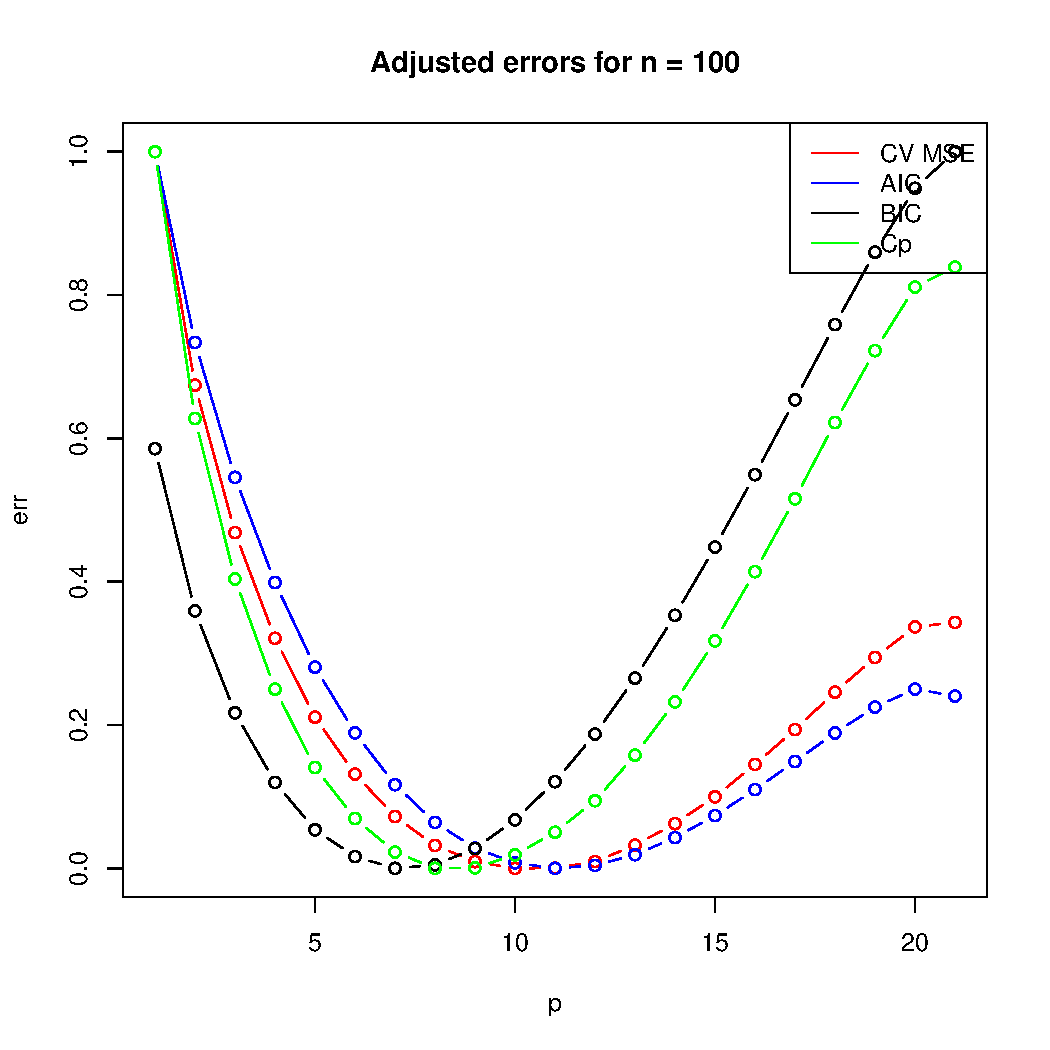
\includegraphics[width=\maxwidth]{figure/unnamed-chunk-5-1} 
\begin{kframe}\begin{alltt}
\hlkwd{plot_err}\hlstd{(Rep_backward1000[}\hlopt{-}\hlkwd{c}\hlstd{(}\hlnum{5}\hlstd{,}\hlnum{6}\hlstd{)],}\hlnum{1000}\hlstd{)}
\end{alltt}
\end{kframe}
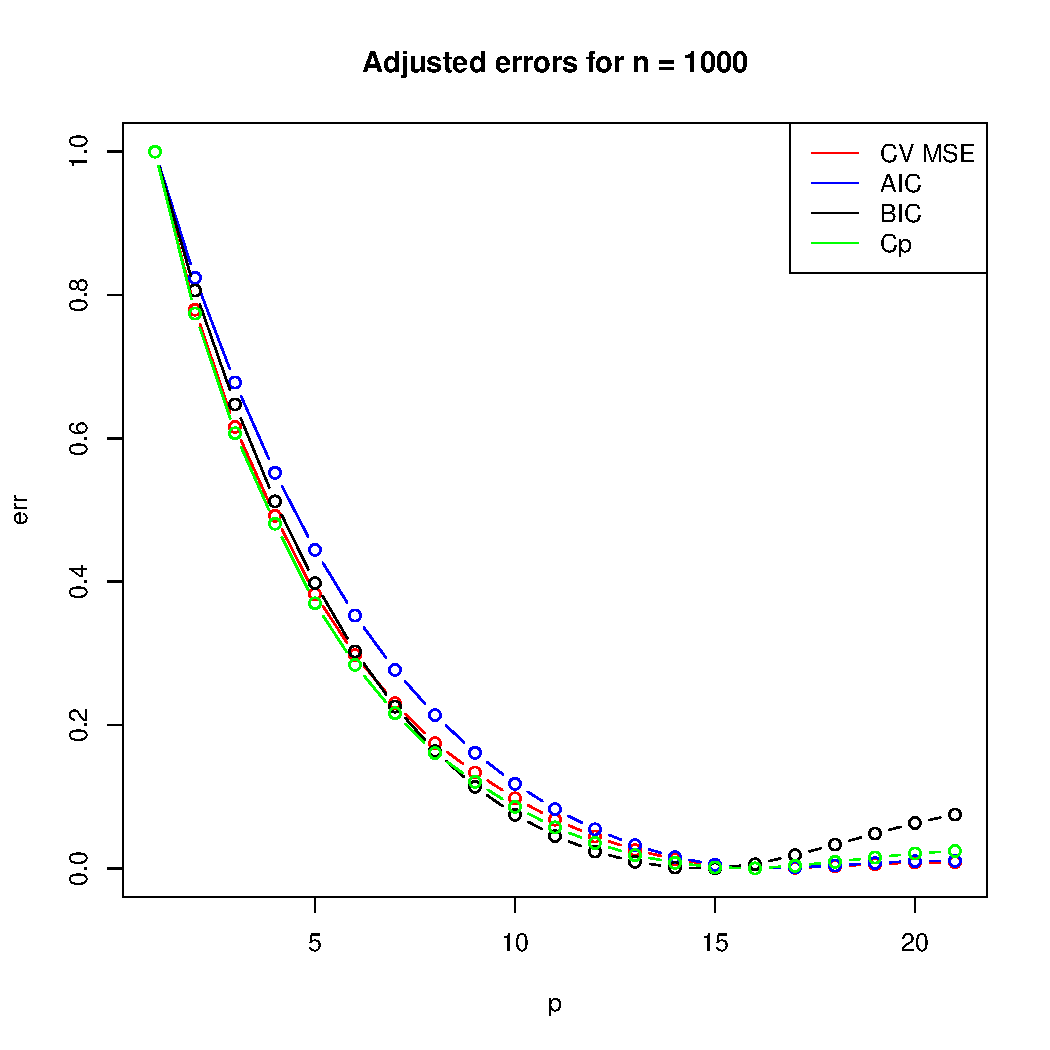
\includegraphics[width=\maxwidth]{figure/unnamed-chunk-5-2} 
\begin{kframe}\begin{alltt}
\hlstd{plot_model_sizes} \hlkwb{=} \hlkwa{function}\hlstd{(}\hlkwc{metrics}\hlstd{,}\hlkwc{n}\hlstd{)\{}
  \hlstd{m} \hlkwb{=} \hlkwd{lapply}\hlstd{(metrics,} \hlkwa{function}\hlstd{(}\hlkwc{X}\hlstd{) \{}\hlkwd{apply}\hlstd{(X,}\hlnum{1}\hlstd{,which.min)\})}
  \hlkwd{par}\hlstd{(}\hlkwc{mfrow}\hlstd{=}\hlkwd{c}\hlstd{(}\hlnum{2}\hlstd{,}\hlnum{2}\hlstd{),}\hlkwc{oma}\hlstd{=}\hlkwd{c}\hlstd{(}\hlnum{0}\hlstd{,}\hlnum{0}\hlstd{,}\hlnum{3}\hlstd{,}\hlnum{0}\hlstd{))}
  \hlkwd{hist}\hlstd{(m}\hlopt{$}\hlstd{MSE,}\hlkwc{main}\hlstd{=}\hlstr{"MSE"}\hlstd{,}\hlkwc{xlim}\hlstd{=}\hlkwd{c}\hlstd{(}\hlnum{0}\hlstd{,}\hlnum{21}\hlstd{),}\hlkwc{breaks}\hlstd{=}\hlnum{0}\hlopt{:}\hlnum{21}\hlstd{,}\hlkwc{xlab}\hlstd{=}\hlstr{"p"}\hlstd{)}
  \hlkwd{hist}\hlstd{(m}\hlopt{$}\hlstd{AIC,}\hlkwc{main}\hlstd{=}\hlstr{"AIC"}\hlstd{,}\hlkwc{xlim}\hlstd{=}\hlkwd{c}\hlstd{(}\hlnum{0}\hlstd{,}\hlnum{21}\hlstd{),}\hlkwc{breaks}\hlstd{=}\hlnum{0}\hlopt{:}\hlnum{21}\hlstd{,}\hlkwc{xlab}\hlstd{=}\hlstr{"p"}\hlstd{)}
  \hlkwd{hist}\hlstd{(m}\hlopt{$}\hlstd{BIC,}\hlkwc{main}\hlstd{=}\hlstr{"BIC"}\hlstd{,}\hlkwc{xlim}\hlstd{=}\hlkwd{c}\hlstd{(}\hlnum{0}\hlstd{,}\hlnum{21}\hlstd{),}\hlkwc{breaks}\hlstd{=}\hlnum{0}\hlopt{:}\hlnum{21}\hlstd{,}\hlkwc{xlab}\hlstd{=}\hlstr{"p"}\hlstd{)}
  \hlkwd{hist}\hlstd{(m}\hlopt{$}\hlstd{Cp ,}\hlkwc{main}\hlstd{=}\hlstr{"Cp "}\hlstd{,}\hlkwc{xlim}\hlstd{=}\hlkwd{c}\hlstd{(}\hlnum{0}\hlstd{,}\hlnum{21}\hlstd{),}\hlkwc{breaks}\hlstd{=}\hlnum{0}\hlopt{:}\hlnum{21}\hlstd{,}\hlkwc{xlab}\hlstd{=}\hlstr{"p"}\hlstd{)}
  \hlkwd{title}\hlstd{(}\hlkwd{paste}\hlstd{(}\hlstr{"Empirical distribution of best model sizes\textbackslash{}nfor n = "}\hlstd{,n),}
        \hlkwc{outer}\hlstd{=}\hlnum{TRUE}\hlstd{)}
  \hlkwd{par}\hlstd{(}\hlkwc{mfrow}\hlstd{=}\hlkwd{c}\hlstd{(}\hlnum{1}\hlstd{,}\hlnum{1}\hlstd{),}\hlkwc{oma}\hlstd{=}\hlkwd{c}\hlstd{(}\hlnum{0}\hlstd{,}\hlnum{0}\hlstd{,}\hlnum{0}\hlstd{,}\hlnum{0}\hlstd{))}
\hlstd{\}}

\hlkwd{plot_model_sizes}\hlstd{(Rep_backward100[}\hlopt{-}\hlkwd{c}\hlstd{(}\hlnum{5}\hlstd{,}\hlnum{6}\hlstd{)],}\hlkwc{n}\hlstd{=}\hlnum{100}\hlstd{)}
\end{alltt}
\end{kframe}
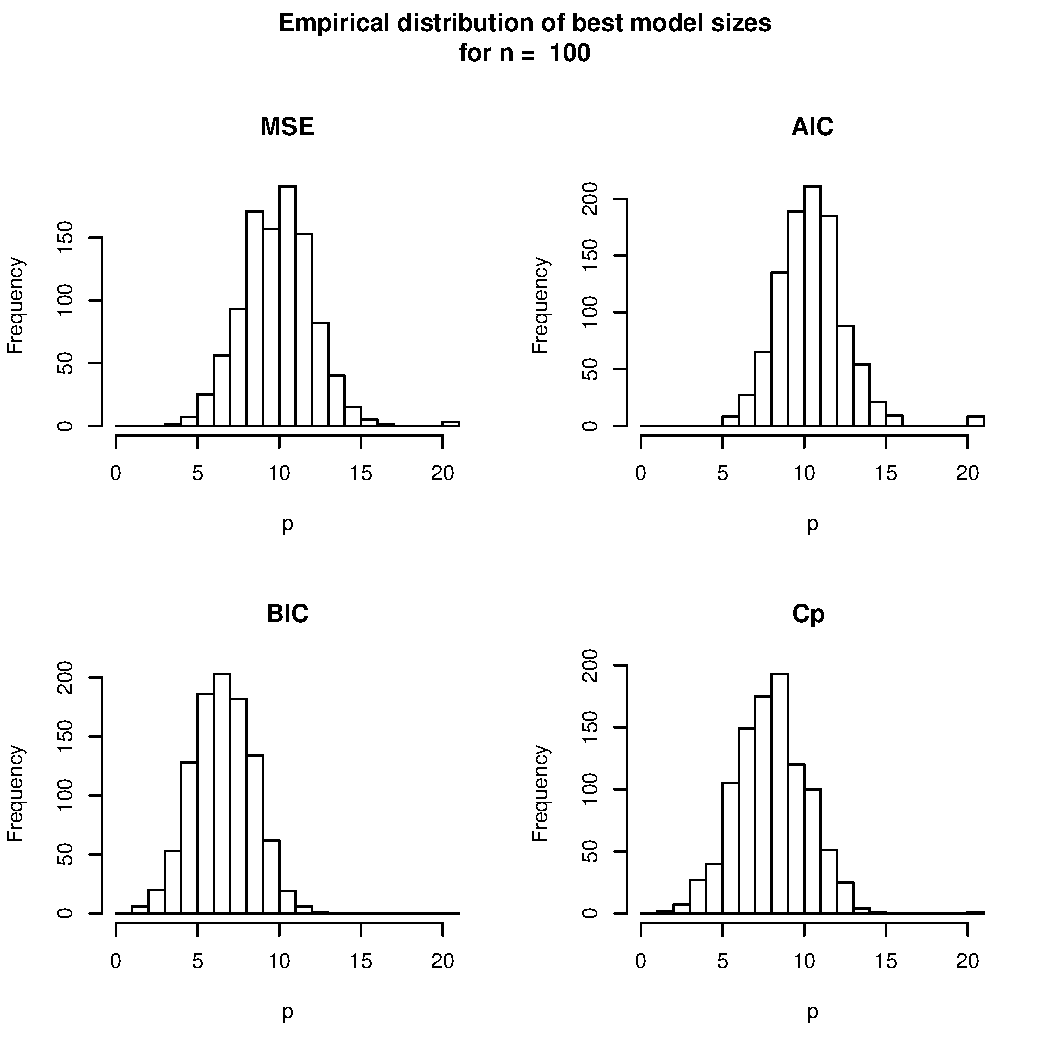
\includegraphics[width=\maxwidth]{figure/unnamed-chunk-5-3} 
\begin{kframe}\begin{alltt}
\hlkwd{plot_model_sizes}\hlstd{(Rep_backward1000[}\hlopt{-}\hlkwd{c}\hlstd{(}\hlnum{5}\hlstd{,}\hlnum{6}\hlstd{)],}\hlkwc{n}\hlstd{=}\hlnum{1000}\hlstd{)}
\end{alltt}
\end{kframe}
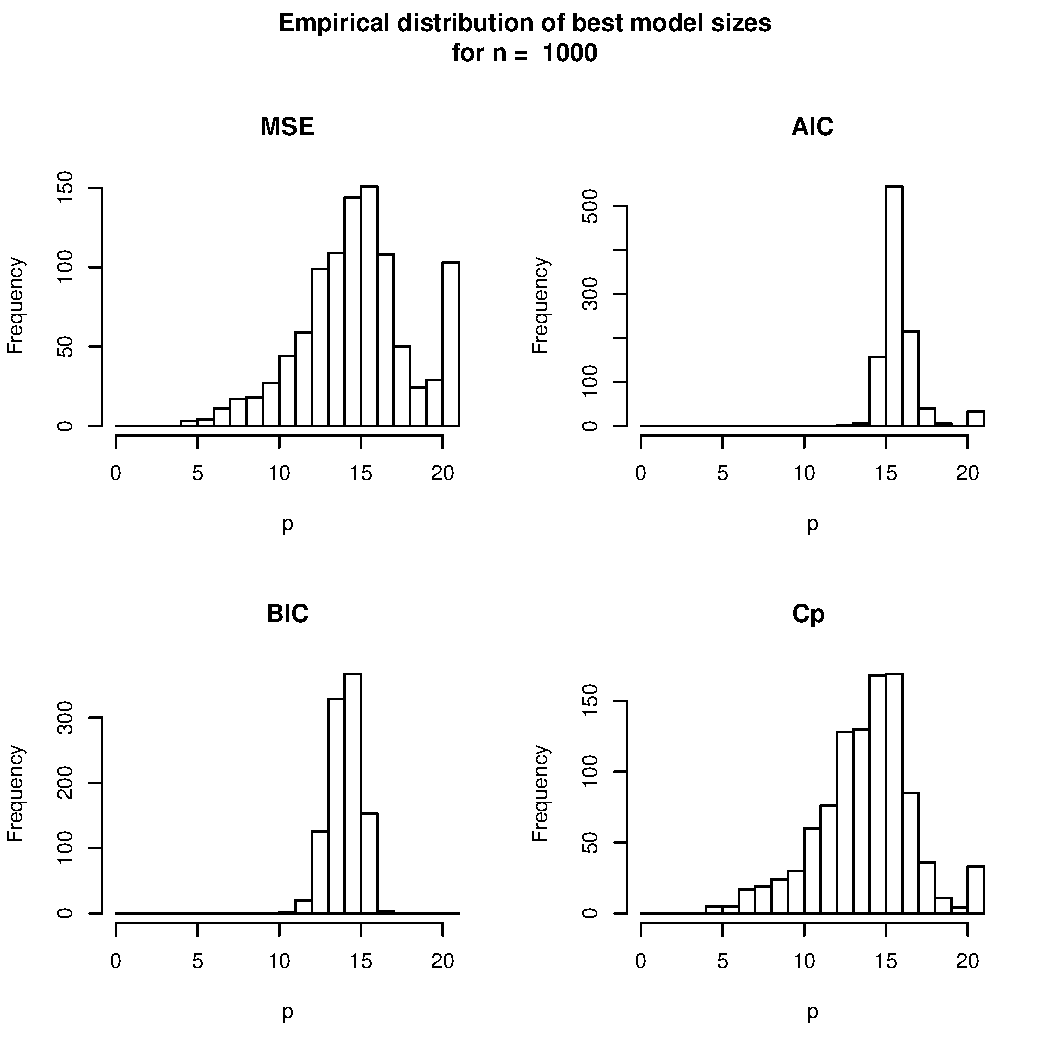
\includegraphics[width=\maxwidth]{figure/unnamed-chunk-5-4} 

\end{knitrout}
\subsection{Proportions}
Here I calculate the proportion of times each coefficient was left out (for the first 15) and put in (for the last 5).
\begin{knitrout}
\definecolor{shadecolor}{rgb}{0.969, 0.969, 0.969}\color{fgcolor}\begin{kframe}
\begin{alltt}
\hlcom{# Proportions -----------------------------------------------}

\hlcom{## # left out first 15}
\hlstd{prop_left} \hlkwb{=} \hlkwa{function}\hlstd{(}\hlkwc{metrics}\hlstd{)\{}
  \hlstd{optimum} \hlkwb{=} \hlkwd{lapply}\hlstd{(metrics[}\hlopt{-}\hlkwd{c}\hlstd{(}\hlnum{5}\hlstd{,}\hlnum{6}\hlstd{)],} \hlkwa{function}\hlstd{(}\hlkwc{X}\hlstd{)}
    \hlstd{\{}\hlkwd{apply}\hlstd{(X,}\hlnum{1}\hlstd{,which.min)\})}
  \hlstd{proportions_left} \hlkwb{=} \hlstd{optimum}
  \hlkwa{for} \hlstd{(i} \hlkwa{in} \hlnum{1}\hlopt{:}\hlstd{B)\{}
    \hlstd{proportions_left}\hlopt{$}\hlstd{MSE[i]} \hlkwb{=} \hlnum{1}\hlopt{-}\hlkwd{length}\hlstd{(}\hlkwd{intersect}\hlstd{(}
      \hlstd{metrics}\hlopt{$}\hlstd{variables[i,}\hlnum{1}\hlopt{:}\hlstd{(optimum}\hlopt{$}\hlstd{MSE[i]}\hlopt{-}\hlnum{1}\hlstd{)],}
      \hlstd{metrics}\hlopt{$}\hlstd{names[i,}\hlnum{1}\hlopt{:}\hlnum{15}\hlstd{]))}\hlopt{/}\hlnum{15}
    \hlstd{proportions_left}\hlopt{$}\hlstd{AIC[i]} \hlkwb{=} \hlnum{1}\hlopt{-}\hlkwd{length}\hlstd{(}\hlkwd{intersect}\hlstd{(}
      \hlstd{metrics}\hlopt{$}\hlstd{variables[i,}\hlnum{1}\hlopt{:}\hlstd{(optimum}\hlopt{$}\hlstd{AIC[i]}\hlopt{-}\hlnum{1}\hlstd{)],}
      \hlstd{metrics}\hlopt{$}\hlstd{names[i,}\hlnum{1}\hlopt{:}\hlnum{15}\hlstd{]))}\hlopt{/}\hlnum{15}
    \hlstd{proportions_left}\hlopt{$}\hlstd{BIC[i]} \hlkwb{=} \hlnum{1}\hlopt{-}\hlkwd{length}\hlstd{(}\hlkwd{intersect}\hlstd{(}
      \hlstd{metrics}\hlopt{$}\hlstd{variables[i,}\hlnum{1}\hlopt{:}\hlstd{(optimum}\hlopt{$}\hlstd{BIC[i]}\hlopt{-}\hlnum{1}\hlstd{)],}
      \hlstd{metrics}\hlopt{$}\hlstd{names[i,}\hlnum{1}\hlopt{:}\hlnum{15}\hlstd{]))}\hlopt{/}\hlnum{15}
    \hlstd{proportions_left}\hlopt{$}\hlstd{Cp[i]} \hlkwb{=}  \hlnum{1}\hlopt{-}\hlkwd{length}\hlstd{(}\hlkwd{intersect}\hlstd{(}
      \hlstd{metrics}\hlopt{$}\hlstd{variables[i,}\hlnum{1}\hlopt{:}\hlstd{(optimum}\hlopt{$}\hlstd{Cp[i]} \hlopt{-}\hlnum{1}\hlstd{)],}
      \hlstd{metrics}\hlopt{$}\hlstd{names[i,}\hlnum{1}\hlopt{:}\hlnum{15}\hlstd{]))}\hlopt{/}\hlnum{15}
  \hlstd{\}}
  \hlstd{proportions_left}
\hlstd{\}}

\hlstd{proportions_left100} \hlkwb{=} \hlkwd{prop_left}\hlstd{(Rep_backward100)}
\hlstd{proportions_left1000} \hlkwb{=} \hlkwd{prop_left}\hlstd{(Rep_backward1000)}


\hlcom{## # kept last 5}
\hlstd{prop_kept} \hlkwb{=} \hlkwa{function}\hlstd{(}\hlkwc{metrics}\hlstd{)\{}
  \hlstd{optimum} \hlkwb{=} \hlkwd{lapply}\hlstd{(metrics[}\hlopt{-}\hlkwd{c}\hlstd{(}\hlnum{5}\hlstd{,}\hlnum{6}\hlstd{)],} \hlkwa{function}\hlstd{(}\hlkwc{X}\hlstd{)}
    \hlstd{\{}\hlkwd{apply}\hlstd{(X,}\hlnum{1}\hlstd{,which.min)\})}
  \hlstd{proportions_kept} \hlkwb{=} \hlstd{optimum}
  \hlkwa{for} \hlstd{(i} \hlkwa{in} \hlnum{1}\hlopt{:}\hlstd{B)\{}
    \hlstd{proportions_kept}\hlopt{$}\hlstd{MSE[i]} \hlkwb{=} \hlkwd{length}\hlstd{(}\hlkwd{intersect}\hlstd{(}
      \hlstd{metrics}\hlopt{$}\hlstd{variables[i,}\hlnum{1}\hlopt{:}\hlstd{(optimum}\hlopt{$}\hlstd{MSE[i]}\hlopt{-}\hlnum{1}\hlstd{)],}
      \hlstd{metrics}\hlopt{$}\hlstd{names[i,}\hlnum{16}\hlopt{:}\hlnum{20}\hlstd{]))}\hlopt{/}\hlnum{5}
    \hlstd{proportions_kept}\hlopt{$}\hlstd{AIC[i]} \hlkwb{=} \hlkwd{length}\hlstd{(}\hlkwd{intersect}\hlstd{(}
      \hlstd{metrics}\hlopt{$}\hlstd{variables[i,}\hlnum{1}\hlopt{:}\hlstd{(optimum}\hlopt{$}\hlstd{AIC[i]}\hlopt{-}\hlnum{1}\hlstd{)],}
      \hlstd{metrics}\hlopt{$}\hlstd{names[i,}\hlnum{16}\hlopt{:}\hlnum{20}\hlstd{]))}\hlopt{/}\hlnum{5}
    \hlstd{proportions_kept}\hlopt{$}\hlstd{BIC[i]} \hlkwb{=} \hlkwd{length}\hlstd{(}\hlkwd{intersect}\hlstd{(}
      \hlstd{metrics}\hlopt{$}\hlstd{variables[i,}\hlnum{1}\hlopt{:}\hlstd{(optimum}\hlopt{$}\hlstd{BIC[i]}\hlopt{-}\hlnum{1}\hlstd{)],}
      \hlstd{metrics}\hlopt{$}\hlstd{names[i,}\hlnum{16}\hlopt{:}\hlnum{20}\hlstd{]))}\hlopt{/}\hlnum{5}
    \hlstd{proportions_kept}\hlopt{$}\hlstd{Cp[i]} \hlkwb{=}  \hlkwd{length}\hlstd{(}\hlkwd{intersect}\hlstd{(}
      \hlstd{metrics}\hlopt{$}\hlstd{variables[i,}\hlnum{1}\hlopt{:}\hlstd{(optimum}\hlopt{$}\hlstd{Cp[i])}\hlopt{-}\hlnum{1} \hlstd{],}
      \hlstd{metrics}\hlopt{$}\hlstd{names[i,}\hlnum{16}\hlopt{:}\hlnum{20}\hlstd{]))}\hlopt{/}\hlnum{5}
  \hlstd{\}}
  \hlstd{proportions_kept}
\hlstd{\}}

\hlstd{proportions_kept100} \hlkwb{=} \hlkwd{prop_kept}\hlstd{(Rep_backward100)}
\hlstd{proportions_kept1000} \hlkwb{=} \hlkwd{prop_kept}\hlstd{(Rep_backward1000)}



\hlcom{# Plot ------------------------------------------------------}

\hlstd{plot_kept} \hlkwb{=} \hlkwa{function}\hlstd{(}\hlkwc{proportions_kept}\hlstd{,}\hlkwc{n}\hlstd{)\{}
  \hlkwd{par}\hlstd{(}\hlkwc{mfrow}\hlstd{=}\hlkwd{c}\hlstd{(}\hlnum{2}\hlstd{,}\hlnum{2}\hlstd{),}\hlkwc{oma}\hlstd{=}\hlkwd{c}\hlstd{(}\hlnum{0}\hlstd{,}\hlnum{0}\hlstd{,}\hlnum{3}\hlstd{,}\hlnum{0}\hlstd{))}
  \hlkwd{hist}\hlstd{(proportions_kept}\hlopt{$}\hlstd{MSE,}\hlkwc{main}\hlstd{=}\hlstr{"MSE"}\hlstd{,}
       \hlkwc{xlim}\hlstd{=}\hlkwd{c}\hlstd{(}\hlnum{0}\hlstd{,}\hlnum{1}\hlstd{),}\hlkwc{xlab}\hlstd{=}\hlstr{"ratio"}\hlstd{)}
  \hlkwd{hist}\hlstd{(proportions_kept}\hlopt{$}\hlstd{AIC,}\hlkwc{main}\hlstd{=}\hlstr{"AIC"}\hlstd{,}
       \hlkwc{xlim}\hlstd{=}\hlkwd{c}\hlstd{(}\hlnum{0}\hlstd{,}\hlnum{1}\hlstd{),}\hlkwc{xlab}\hlstd{=}\hlstr{"ratio"}\hlstd{)}
  \hlkwd{hist}\hlstd{(proportions_kept}\hlopt{$}\hlstd{BIC,}\hlkwc{main}\hlstd{=}\hlstr{"BIC"}\hlstd{,}
       \hlkwc{xlim}\hlstd{=}\hlkwd{c}\hlstd{(}\hlnum{0}\hlstd{,}\hlnum{1}\hlstd{),}\hlkwc{xlab}\hlstd{=}\hlstr{"ratio"}\hlstd{)}
  \hlkwd{hist}\hlstd{(proportions_kept}\hlopt{$}\hlstd{Cp,} \hlkwc{main}\hlstd{=}\hlstr{"Cp"}\hlstd{,}
       \hlkwc{xlim}\hlstd{=}\hlkwd{c}\hlstd{(}\hlnum{0}\hlstd{,}\hlnum{1}\hlstd{),}\hlkwc{xlab}\hlstd{=} \hlstr{"ratio"}\hlstd{)}
  \hlkwd{title}\hlstd{(}\hlkwd{paste}\hlstd{(}\hlstr{"Proportion of times each coefficient was put in\textbackslash{}nfor n = "}\hlstd{,n),}
        \hlkwc{outer}\hlstd{=}\hlnum{TRUE}\hlstd{)}
  \hlkwd{par}\hlstd{(}\hlkwc{mfrow}\hlstd{=}\hlkwd{c}\hlstd{(}\hlnum{1}\hlstd{,}\hlnum{1}\hlstd{),}\hlkwc{oma}\hlstd{=}\hlkwd{c}\hlstd{(}\hlnum{0}\hlstd{,}\hlnum{0}\hlstd{,}\hlnum{0}\hlstd{,}\hlnum{0}\hlstd{))}
\hlstd{\}}

\hlkwd{plot_kept}\hlstd{(proportions_kept100,}\hlnum{100}\hlstd{)}
\end{alltt}
\end{kframe}
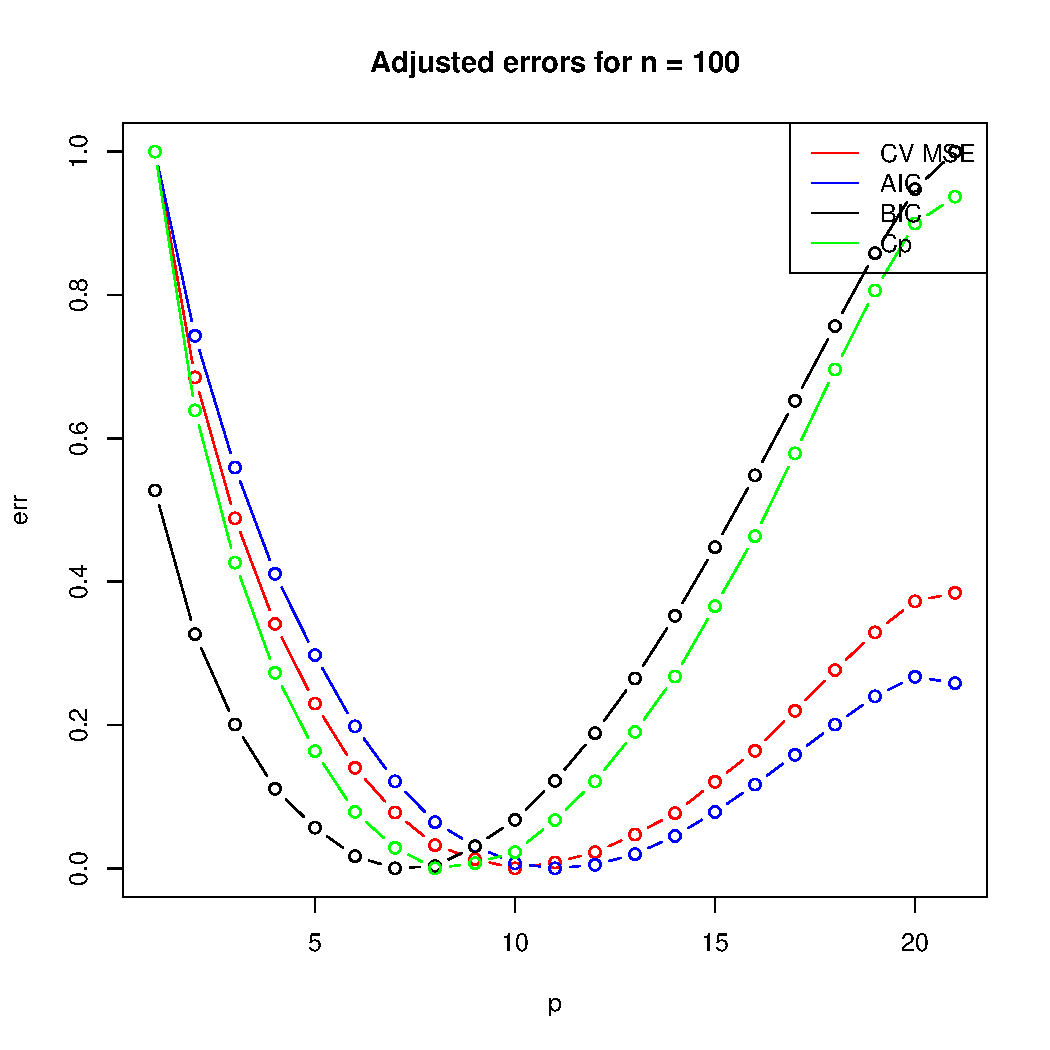
\includegraphics[width=\maxwidth]{figure/unnamed-chunk-6-1} 
\begin{kframe}\begin{alltt}
\hlkwd{plot_kept}\hlstd{(proportions_kept1000,}\hlnum{1000}\hlstd{)}
\end{alltt}
\end{kframe}
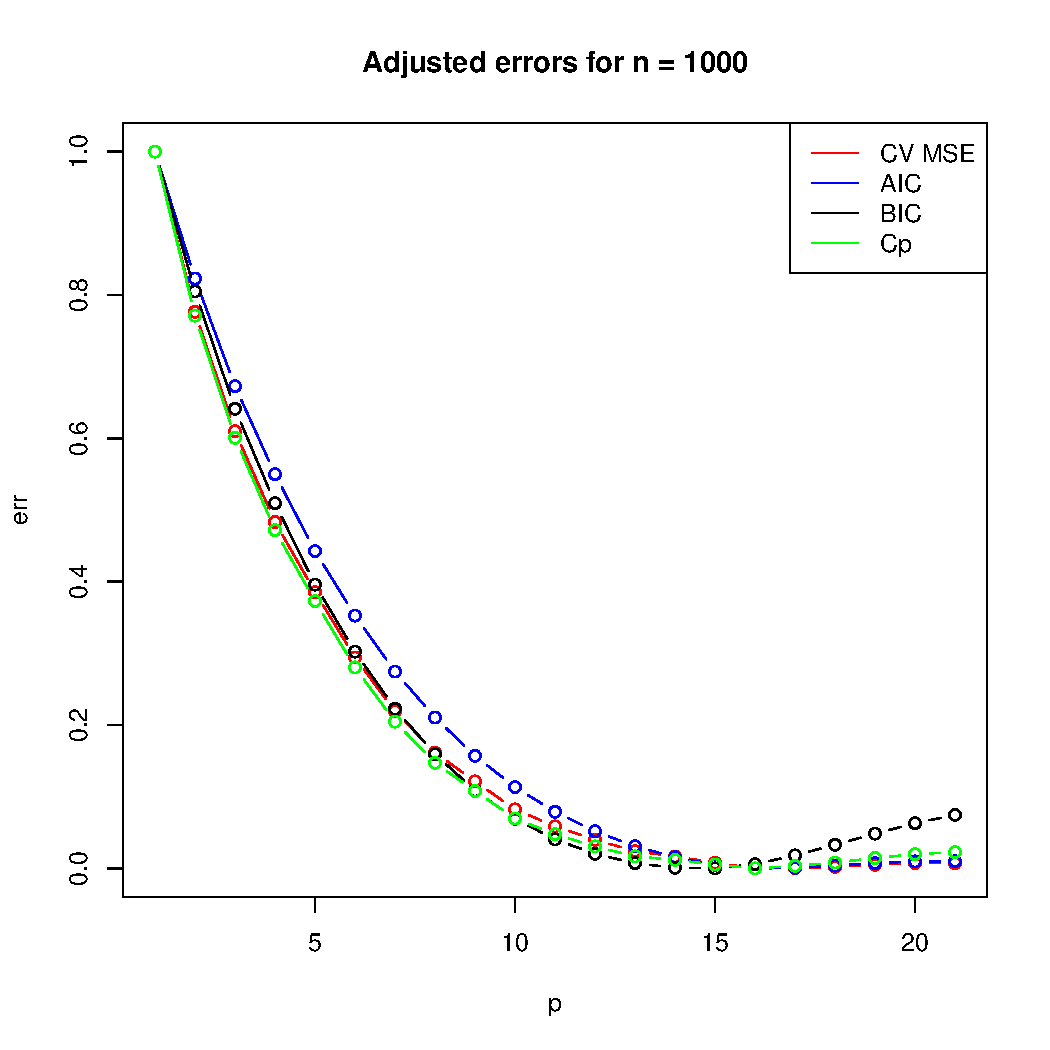
\includegraphics[width=\maxwidth]{figure/unnamed-chunk-6-2} 
\begin{kframe}\begin{alltt}
\hlstd{plot_left} \hlkwb{=} \hlkwa{function}\hlstd{(}\hlkwc{proportions_left}\hlstd{,}\hlkwc{n}\hlstd{)\{}
  \hlkwd{par}\hlstd{(}\hlkwc{mfrow}\hlstd{=}\hlkwd{c}\hlstd{(}\hlnum{2}\hlstd{,}\hlnum{2}\hlstd{),}\hlkwc{oma}\hlstd{=}\hlkwd{c}\hlstd{(}\hlnum{0}\hlstd{,}\hlnum{0}\hlstd{,}\hlnum{3}\hlstd{,}\hlnum{0}\hlstd{))}
  \hlkwd{hist}\hlstd{(proportions_left}\hlopt{$}\hlstd{MSE,}\hlkwc{main}\hlstd{=}\hlstr{"MSE"}\hlstd{,}\hlkwc{xlim}\hlstd{=}\hlkwd{c}\hlstd{(}\hlnum{0}\hlstd{,}\hlnum{1}\hlstd{),}\hlkwc{xlab}\hlstd{=}\hlstr{"ratio"}\hlstd{)}
  \hlkwd{hist}\hlstd{(proportions_left}\hlopt{$}\hlstd{AIC,}\hlkwc{main}\hlstd{=}\hlstr{"AIC"}\hlstd{,}\hlkwc{xlim}\hlstd{=}\hlkwd{c}\hlstd{(}\hlnum{0}\hlstd{,}\hlnum{1}\hlstd{),}\hlkwc{xlab}\hlstd{=}\hlstr{"ratio"}\hlstd{)}
  \hlkwd{hist}\hlstd{(proportions_left}\hlopt{$}\hlstd{BIC,}\hlkwc{main}\hlstd{=}\hlstr{"BIC"}\hlstd{,}\hlkwc{xlim}\hlstd{=}\hlkwd{c}\hlstd{(}\hlnum{0}\hlstd{,}\hlnum{1}\hlstd{),}\hlkwc{xlab}\hlstd{=}\hlstr{"ratio"}\hlstd{)}
  \hlkwd{hist}\hlstd{(proportions_left}\hlopt{$}\hlstd{Cp,} \hlkwc{main}\hlstd{=}\hlstr{"Cp"}\hlstd{,}\hlkwc{xlim}\hlstd{=}\hlkwd{c}\hlstd{(}\hlnum{0}\hlstd{,}\hlnum{1}\hlstd{),}\hlkwc{xlab}\hlstd{=} \hlstr{"ratio"}\hlstd{)}
  \hlkwd{title}\hlstd{(}\hlkwd{paste}\hlstd{(}\hlstr{"Proportion of times each coefficient was left out\textbackslash{}nfor n = "}\hlstd{,n),}
        \hlkwc{outer}\hlstd{=}\hlnum{TRUE}\hlstd{)}
  \hlkwd{par}\hlstd{(}\hlkwc{mfrow}\hlstd{=}\hlkwd{c}\hlstd{(}\hlnum{1}\hlstd{,}\hlnum{1}\hlstd{),}\hlkwc{oma}\hlstd{=}\hlkwd{c}\hlstd{(}\hlnum{0}\hlstd{,}\hlnum{0}\hlstd{,}\hlnum{0}\hlstd{,}\hlnum{0}\hlstd{))}
\hlstd{\}}

\hlkwd{plot_left}\hlstd{(proportions_left100,}\hlnum{100}\hlstd{)}
\end{alltt}
\end{kframe}
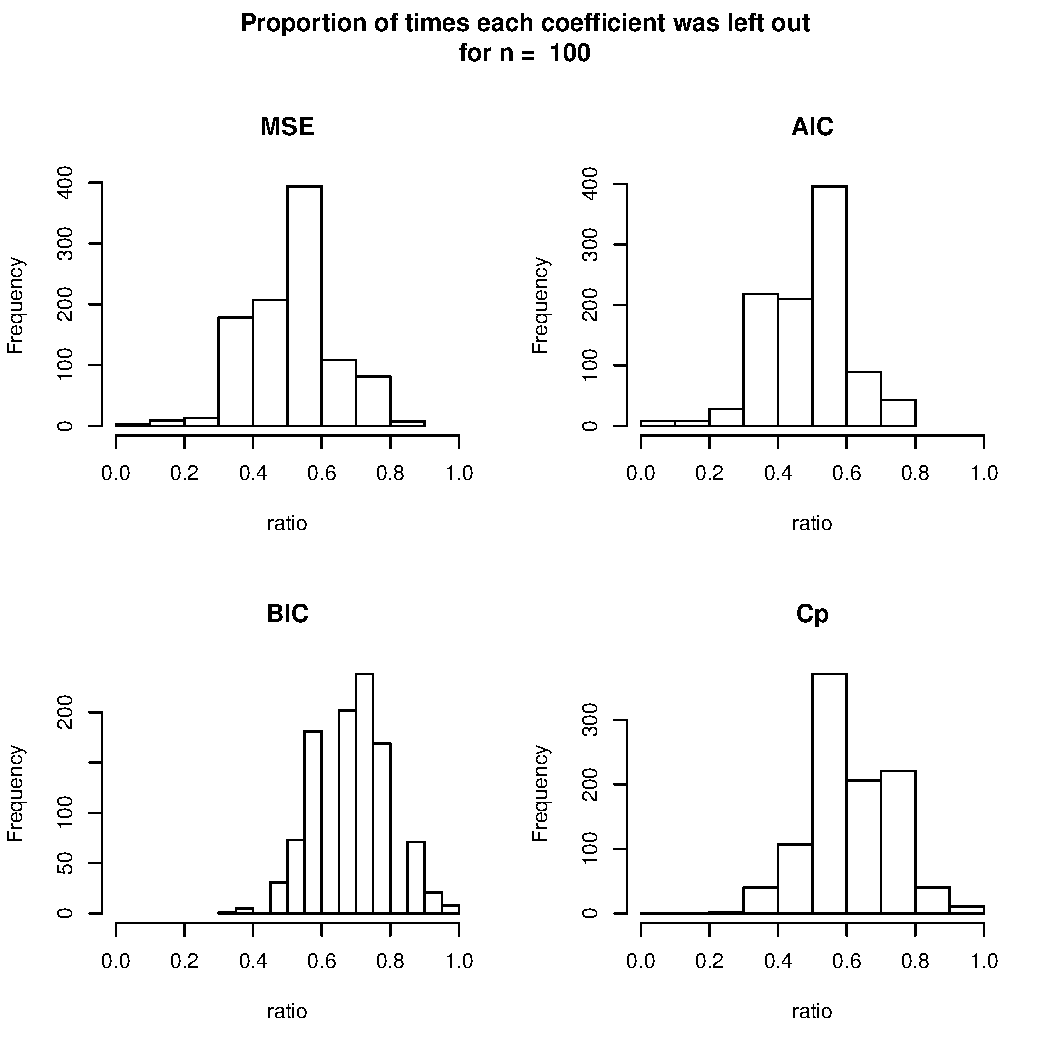
\includegraphics[width=\maxwidth]{figure/unnamed-chunk-6-3} 
\begin{kframe}\begin{alltt}
\hlkwd{plot_left}\hlstd{(proportions_left1000,}\hlnum{1000}\hlstd{)}
\end{alltt}
\end{kframe}
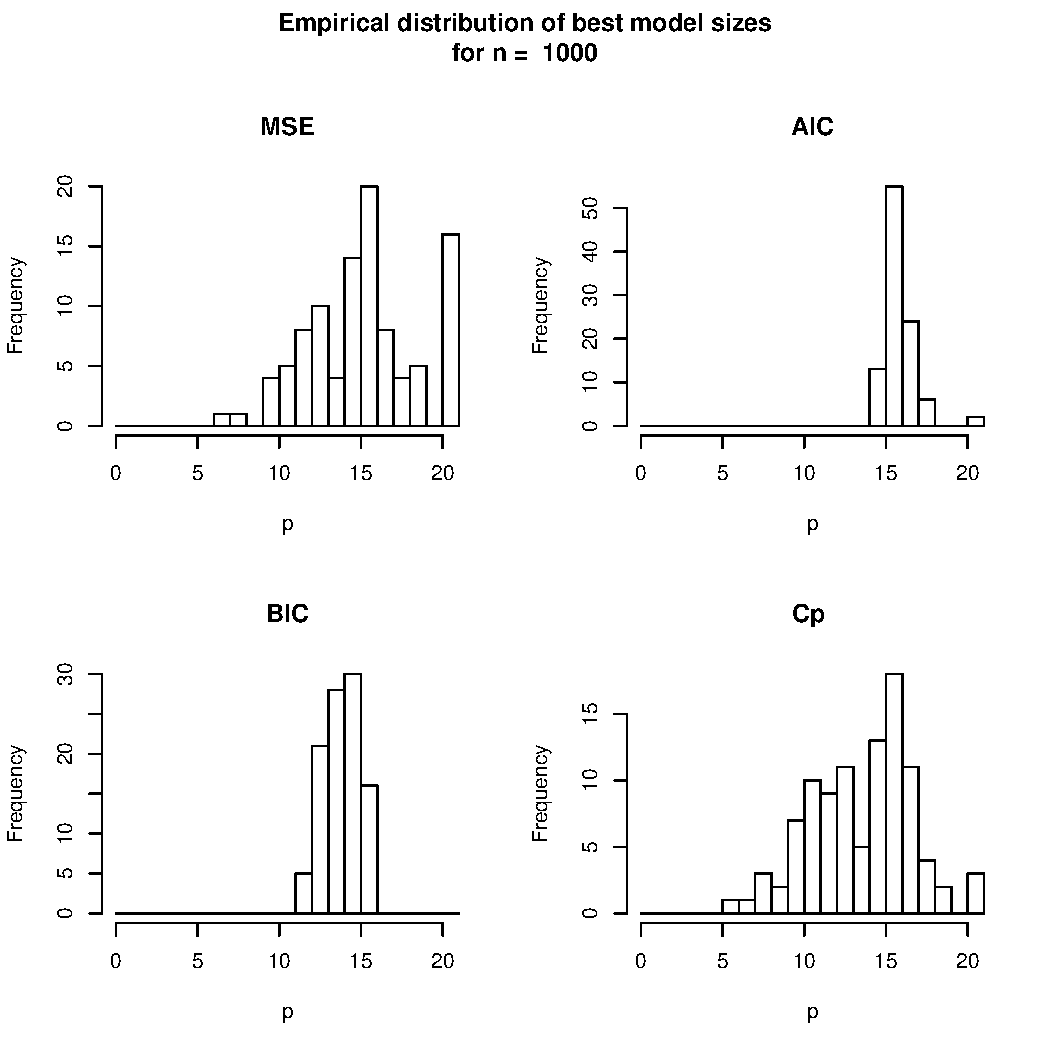
\includegraphics[width=\maxwidth]{figure/unnamed-chunk-6-4} 

\end{knitrout}
BIC has a heavier penalty term than AIC or Cp so it tends to favor simpler models, we can see it here: the proportion of left out parameters for the first 15 variables is greater for this statistic. This is also similar to Mallow’s Cp. AIC has the lowest error, as expected because it favors more complex models than BIC.We can also notice that as n increases, the empirical variance reduces.

\section{}
\subsection{Load data}
Here I load the data with outputing the true beta.
\begin{knitrout}
\definecolor{shadecolor}{rgb}{0.969, 0.969, 0.969}\color{fgcolor}\begin{kframe}
\begin{alltt}
\hlkwd{library}\hlstd{(pls)}
\end{alltt}


{\ttfamily\noindent\itshape\color{messagecolor}{\#\# \\\#\# Attaching package: 'pls'\\\#\# \\\#\# The following object is masked from 'package:stats':\\\#\# \\\#\#\ \ \ \  loadings}}\begin{alltt}
\hlkwd{rm}\hlstd{(}\hlkwc{list} \hlstd{=} \hlkwd{ls}\hlstd{())}
\hlkwd{cat}\hlstd{(}\hlstr{"\textbackslash{}014"}\hlstd{)}
\end{alltt}
\end{kframe}\begin{kframe}\begin{alltt}
\hlcom{# Data --------------------------------------------------}

\hlstd{makedata}\hlkwb{=}\hlkwa{function}\hlstd{(}\hlkwc{p}\hlstd{=}\hlnum{20}\hlstd{,}\hlkwc{wh}\hlstd{=}\hlnum{15}\hlstd{,}\hlkwc{n}\hlstd{=}\hlnum{100}\hlstd{)\{}
  \hlstd{X}\hlkwb{=}\hlkwd{matrix}\hlstd{(}\hlkwd{rnorm}\hlstd{(n}\hlopt{*}\hlstd{p),n,p)}
  \hlstd{exps}\hlkwb{=}\hlkwd{seq}\hlstd{(}\hlopt{-}\hlnum{1}\hlstd{,}\hlopt{-}\hlnum{2.5}\hlstd{,}\hlkwc{length}\hlstd{=wh)}
  \hlstd{beta}\hlkwb{=}\hlkwd{rep}\hlstd{(}\hlnum{0}\hlstd{,p)}
  \hlstd{beta[}\hlnum{1}\hlopt{:}\hlstd{wh]}\hlkwb{=}\hlkwd{exp}\hlstd{(exps)}
  \hlstd{Y}\hlkwb{=}\hlnum{.5}\hlopt{+}\hlstd{X}\hlopt\hlstd{beta}\hlopt{+}\hlkwd{rnorm}\hlstd{(n)}
  \hlstd{data} \hlkwb{=} \hlkwd{data.frame}\hlstd{(Y,X)}
  \hlkwd{colnames}\hlstd{(data)}\hlkwb{=}\hlkwd{c}\hlstd{(}\hlstr{"Y"}\hlstd{,letters[}\hlnum{1}\hlopt{:}\hlnum{20}\hlstd{])}
  \hlstd{switch}\hlkwb{=}\hlkwd{sample}\hlstd{(}\hlnum{20}\hlstd{)}\hlopt{+}\hlnum{1}
  \hlstd{data}\hlkwb{=}\hlstd{data[,}\hlkwd{c}\hlstd{(}\hlnum{1}\hlstd{,switch)]}
  \hlkwd{names}\hlstd{(beta)}\hlkwb{=}\hlkwd{names}\hlstd{(data)[switch]}
  \hlkwd{return}\hlstd{(}\hlkwd{list}\hlstd{(}\hlkwc{df}\hlstd{=data,}\hlkwc{beta}\hlstd{=beta))}
\hlstd{\}}

\hlkwd{set.seed}\hlstd{(}\hlnum{1}\hlstd{)}
\hlstd{data}\hlkwb{=}\hlkwd{makedata}\hlstd{()}
\hlstd{data}\hlopt{$}\hlstd{beta}
\end{alltt}
\begin{verbatim}
##          c          i          g          r          d          o 
## 0.36787944 0.33050190 0.29692203 0.26675395 0.23965104 0.21530185 
##          n          h          m          j          f          q 
## 0.19342660 0.17377394 0.15611805 0.14025603 0.12600565 0.11320313 
##          e          p          s          l          b          a 
## 0.10170139 0.09136826 0.08208500 0.00000000 0.00000000 0.00000000 
##          t          k 
## 0.00000000 0.00000000
\end{verbatim}
\end{kframe}
\end{knitrout}
\subsection{Replicate}
Here again I make use of parrallelization.
\begin{knitrout}
\definecolor{shadecolor}{rgb}{0.969, 0.969, 0.969}\color{fgcolor}\begin{kframe}
\begin{alltt}
\hlcom{# Replicate ------------------------------------------------}
\hlstd{cv_pcr} \hlkwb{=} \hlkwa{function}\hlstd{(}\hlkwc{n}\hlstd{)\{}
  \hlstd{data} \hlkwb{=} \hlkwd{makedata}\hlstd{(}\hlkwc{n}\hlstd{=n)}
  \hlstd{df} \hlkwb{=} \hlstd{data}\hlopt{$}\hlstd{df}
  \hlstd{beta0} \hlkwb{=} \hlstd{data}\hlopt{$}\hlstd{beta}
  \hlstd{pcr.fit} \hlkwb{=} \hlkwd{pcr}\hlstd{(Y}\hlopt{~}\hlnum{0}\hlopt{+}\hlstd{.,} \hlkwc{ncomp}\hlstd{=}\hlnum{20}\hlstd{,} \hlkwc{data}\hlstd{=df,} \hlkwc{validation} \hlstd{=}\hlstr{"CV"}\hlstd{)}
  \hlstd{cv_error} \hlkwb{=} \hlkwd{as.data.frame}\hlstd{(}\hlkwd{RMSEP}\hlstd{(pcr.fit)}\hlopt{$}\hlstd{val)[}\hlnum{1}\hlstd{,]}
  \hlkwd{names}\hlstd{(cv_error)} \hlkwb{=} \hlnum{0}\hlopt{:}\hlnum{20}
  \hlcom{# beta pcr}
  \hlstd{beta0} \hlkwb{=} \hlstd{data}\hlopt{$}\hlstd{beta}
  \hlstd{beta_pcr} \hlkwb{=} \hlkwd{rev}\hlstd{(}\hlkwd{sort}\hlstd{(pcr.fit}\hlopt{$}\hlstd{coefficients[,,}\hlnum{20}\hlstd{]))}
  \hlkwd{return}\hlstd{(}\hlkwd{list}\hlstd{(}\hlkwc{CV}\hlstd{=cv_error,} \hlkwc{beta0}\hlstd{=beta0,} \hlkwc{beta}\hlstd{=beta_pcr))}
\hlstd{\}}


\hlkwd{library}\hlstd{(parallel)}

\hlstd{pcr_rep} \hlkwb{=} \hlkwa{function}\hlstd{(}\hlkwc{B}\hlstd{,}\hlkwc{n}\hlstd{=}\hlnum{100}\hlstd{)\{}
  \hlstd{ncores} \hlkwb{=} \hlkwd{detectCores}\hlstd{()}\hlopt{-}\hlnum{1}
  \hlkwd{print}\hlstd{(}\hlkwd{paste}\hlstd{(}\hlstr{'Starting '}\hlstd{, ncores,} \hlstr{' cores...'}\hlstd{))}
  \hlstd{cl} \hlkwb{=} \hlkwd{makeCluster}\hlstd{(ncores)}
  \hlkwd{clusterEvalQ}\hlstd{(cl,}\hlkwd{library}\hlstd{(pls))}
  \hlkwd{clusterExport}\hlstd{(cl,}\hlkwd{list}\hlstd{(}\hlstr{"cv_pcr"}\hlstd{,}\hlstr{"makedata"}\hlstd{))}
  \hlstd{R} \hlkwb{=} \hlkwd{parSapply}\hlstd{(cl,} \hlnum{1}\hlopt{:}\hlstd{B,} \hlkwa{function}\hlstd{(}\hlkwc{i}\hlstd{,}\hlkwc{...}\hlstd{)}
  \hlstd{\{} \hlkwd{cv_pcr}\hlstd{(}\hlkwc{n}\hlstd{=n) \} )}
  \hlstd{CV} \hlkwb{=} \hlkwd{matrix}\hlstd{(}\hlkwd{unlist}\hlstd{(R[}\hlstr{"CV"}\hlstd{,]),} \hlkwc{nrow} \hlstd{= B,} \hlkwc{byrow} \hlstd{= T)}
  \hlstd{beta0} \hlkwb{=} \hlkwd{matrix}\hlstd{(}\hlkwd{unlist}\hlstd{(R[}\hlstr{"beta0"}\hlstd{,]),} \hlkwc{nrow} \hlstd{= B,} \hlkwc{byrow} \hlstd{= T)[}\hlnum{1}\hlstd{,]}
  \hlstd{beta} \hlkwb{=} \hlkwd{matrix}\hlstd{(}\hlkwd{unlist}\hlstd{(R[}\hlstr{"beta"}\hlstd{,]),} \hlkwc{nrow} \hlstd{= B,} \hlkwc{byrow} \hlstd{= T)}
  \hlkwd{stopCluster}\hlstd{(cl)}
  \hlkwd{print}\hlstd{(}\hlstr{'Done.'}\hlstd{)}
  \hlkwd{return}\hlstd{(}\hlkwd{list}\hlstd{(}\hlkwc{CV}\hlstd{=CV,}\hlkwc{beta}\hlstd{=beta,}\hlkwc{beta0}\hlstd{=beta0))}
\hlstd{\}}

\hlstd{B} \hlkwb{=} \hlnum{1000}
\hlstd{Rep_pcr100} \hlkwb{=} \hlkwd{pcr_rep}\hlstd{(B,}\hlkwc{n}\hlstd{=}\hlnum{100}\hlstd{)}
\end{alltt}
\begin{verbatim}
## [1] "Starting  39  cores..."
## [1] "Done."
\end{verbatim}
\begin{alltt}
\hlstd{Rep_pcr1000} \hlkwb{=} \hlkwd{pcr_rep}\hlstd{(B,}\hlkwc{n}\hlstd{=}\hlnum{1000}\hlstd{)}
\end{alltt}
\begin{verbatim}
## [1] "Starting  39  cores..."
## [1] "Done."
\end{verbatim}
\end{kframe}
\end{knitrout}
\subsection{Plots}
\begin{knitrout}
\definecolor{shadecolor}{rgb}{0.969, 0.969, 0.969}\color{fgcolor}\begin{kframe}
\begin{alltt}
\hlcom{# Plot -----------------------------------------------------}

\hlcom{# n=100}
\hlkwd{boxplot}\hlstd{(Rep_pcr100}\hlopt{$}\hlstd{CV,}
        \hlkwc{main}\hlstd{=}\hlkwd{paste}\hlstd{(}\hlstr{"CV error for PCR with n = "}\hlstd{,}\hlnum{100}\hlstd{),}
        \hlkwc{xlab} \hlstd{=} \hlstr{"Number of components"}\hlstd{,}
        \hlkwc{ylab}\hlstd{=}\hlstr{"test error"}\hlstd{,}\hlkwc{names}\hlstd{=}\hlnum{0}\hlopt{:}\hlnum{20}\hlstd{)}
\end{alltt}
\end{kframe}
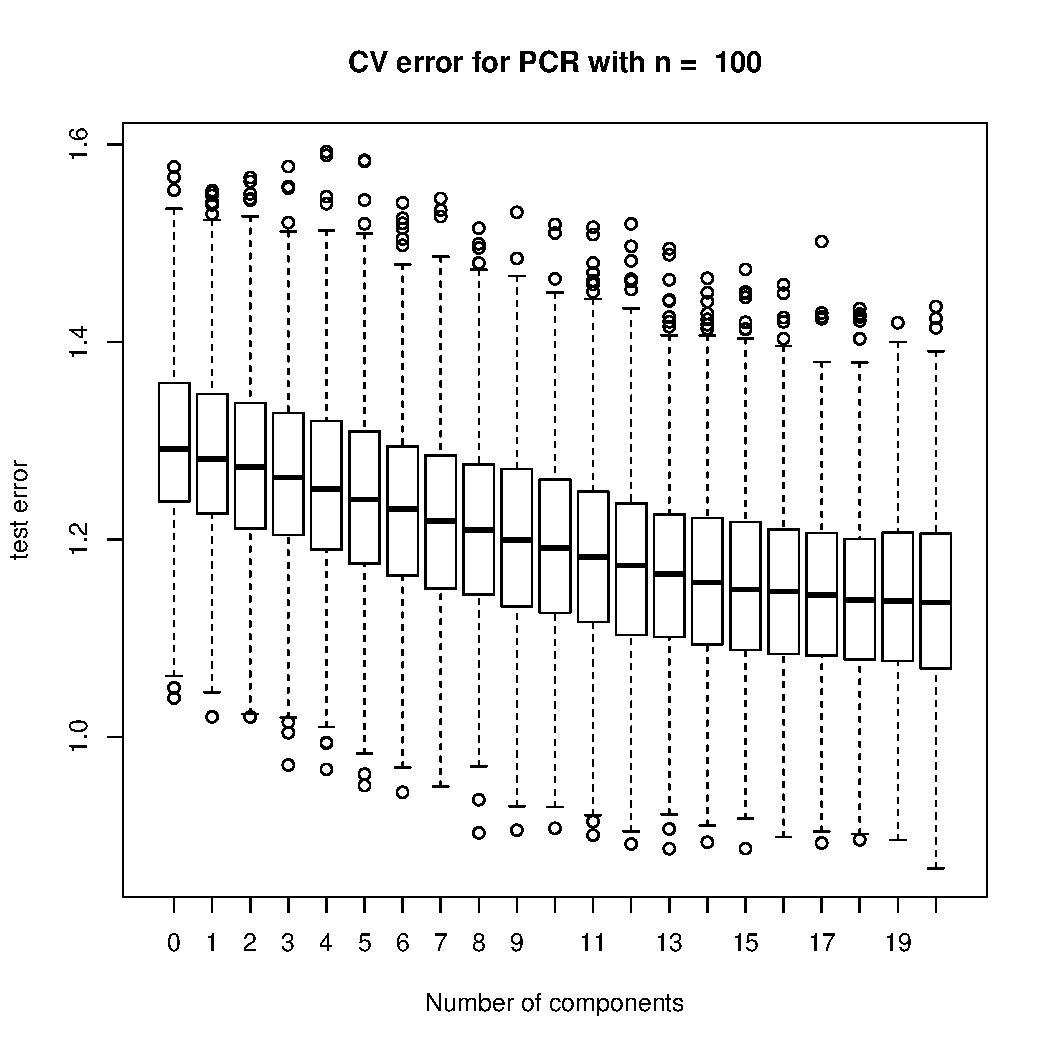
\includegraphics[width=\maxwidth]{figure/unnamed-chunk-9-1} 
\begin{kframe}\begin{alltt}
\hlcom{#n=1000}
\hlkwd{boxplot}\hlstd{(Rep_pcr1000}\hlopt{$}\hlstd{CV,}
        \hlkwc{main}\hlstd{=}\hlkwd{paste}\hlstd{(}\hlstr{"CV error for PCR with n = "}\hlstd{,}\hlnum{1000}\hlstd{),}
        \hlkwc{xlab} \hlstd{=} \hlstr{"Number of components"}\hlstd{,}
        \hlkwc{ylab}\hlstd{=}\hlstr{"test error"}\hlstd{,}\hlkwc{names}\hlstd{=}\hlnum{0}\hlopt{:}\hlnum{20}\hlstd{)}
\end{alltt}
\end{kframe}
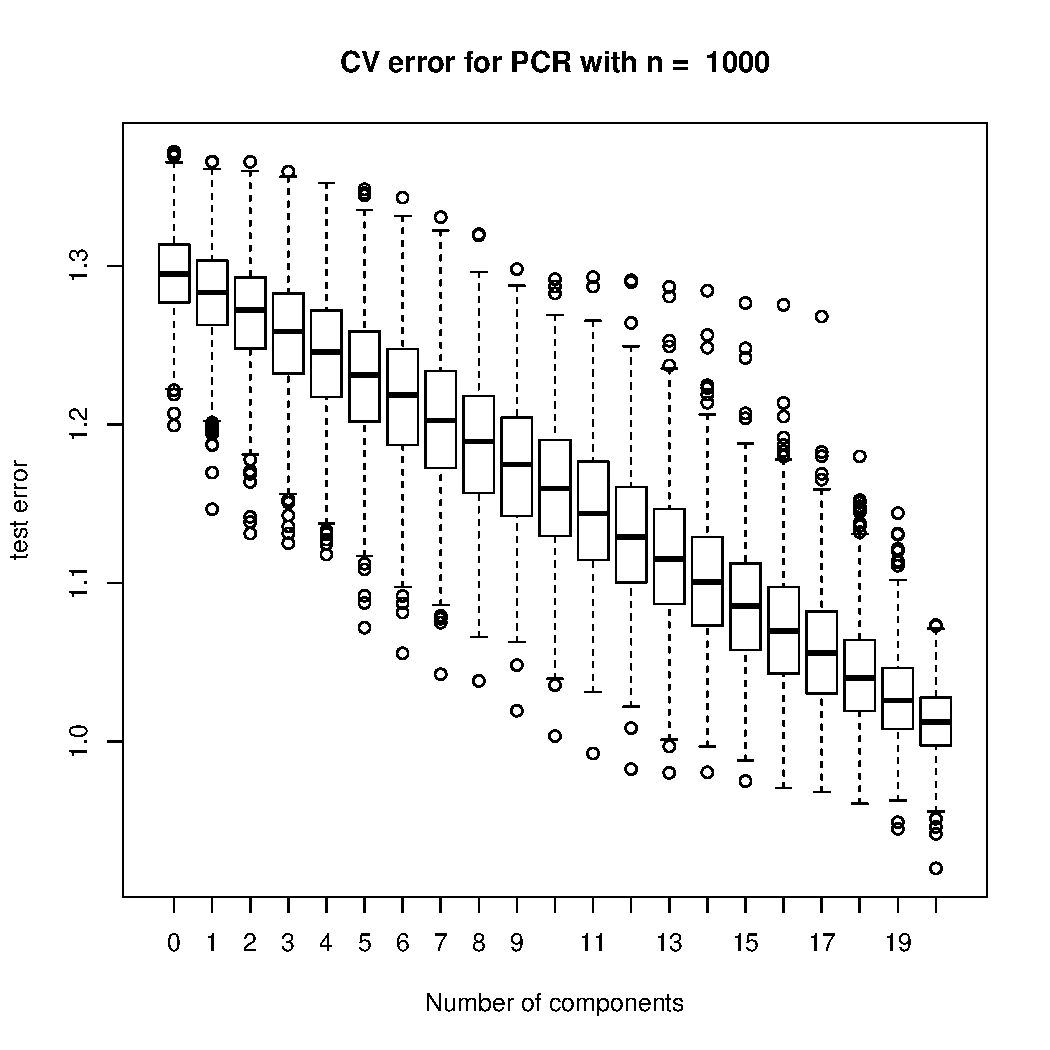
\includegraphics[width=\maxwidth]{figure/unnamed-chunk-9-2} 
\begin{kframe}\begin{alltt}
\hlcom{#n=100}
\hlkwd{boxplot}\hlstd{(Rep_pcr100}\hlopt{$}\hlstd{beta,}
        \hlkwc{main}\hlstd{=}\hlkwd{paste}\hlstd{(}\hlstr{"beta_hat for PCR with n = "}\hlstd{,}\hlnum{100}\hlstd{),}
        \hlkwc{xlab} \hlstd{=} \hlstr{"Number of components"}\hlstd{,}
        \hlkwc{ylab}\hlstd{=}\hlstr{"beta"}\hlstd{)}
\hlkwd{points}\hlstd{(}\hlnum{1}\hlopt{:}\hlnum{20}\hlstd{,Rep_pcr1000}\hlopt{$}\hlstd{beta0,}\hlkwc{col}\hlstd{=}\hlstr{"red"}\hlstd{)}
\end{alltt}
\end{kframe}
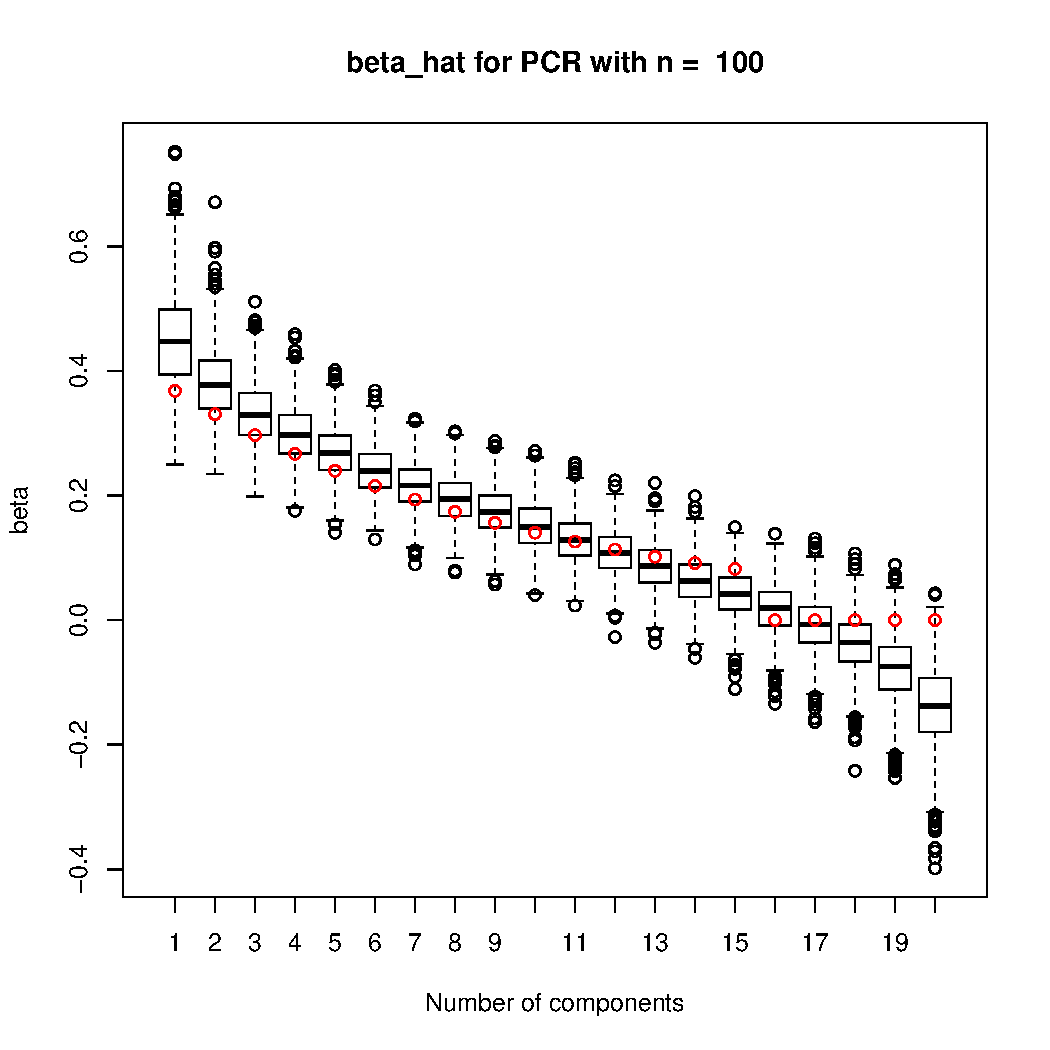
\includegraphics[width=\maxwidth]{figure/unnamed-chunk-9-3} 
\begin{kframe}\begin{alltt}
\hlcom{#n=1000}
\hlkwd{boxplot}\hlstd{(Rep_pcr1000}\hlopt{$}\hlstd{beta,}
        \hlkwc{main}\hlstd{=}\hlkwd{paste}\hlstd{(}\hlstr{"beta_hat for PCR with n = "}\hlstd{,}\hlnum{1000}\hlstd{),}
        \hlkwc{xlab} \hlstd{=} \hlstr{"Number of components"}\hlstd{,}
        \hlkwc{ylab}\hlstd{=}\hlstr{"beta"}\hlstd{)}
\hlkwd{points}\hlstd{(}\hlnum{1}\hlopt{:}\hlnum{20}\hlstd{,Rep_pcr1000}\hlopt{$}\hlstd{beta0,}\hlkwc{col}\hlstd{=}\hlstr{"red"}\hlstd{)}
\end{alltt}
\end{kframe}
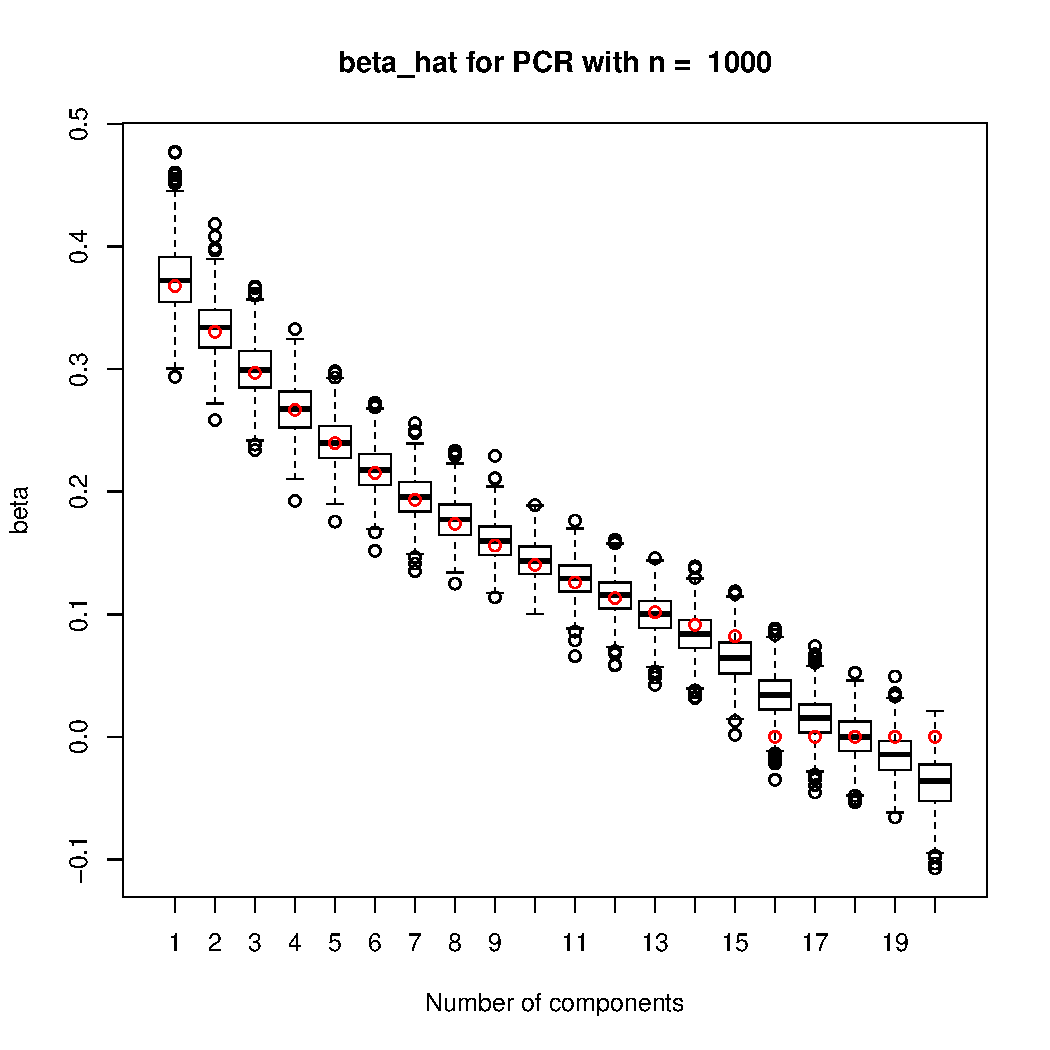
\includegraphics[width=\maxwidth]{figure/unnamed-chunk-9-4} 

\end{knitrout}
The CV error goes down as we increase the number of components. The true beta remains in the confidence interval even if there seems to be a little biased.

\end{document}









